\chapter{Einleitung}

\section{Über KaVo Dental}

\vspace{-1em}  % pull figure closer to text above
\begin{figure}[H]
    \centering
    \includegraphics[height=0.29\textheight]{images/HR-Außenansicht-dunkel.png}
    \caption{KaVo Dental Hauptsitz in Biberach an der Riß}
    \label{fig:kavo_headquarters}
\end{figure}

Die KaVo Dental GmbH mit Hauptsitz in Biberach an der Riß ist ein international führendes Medizintechnikunternehmen, das seit über 110 Jahren in der Dentalbranche steht. Das Unternehmen entwickelt, produziert und vertreibt ein breites Spektrum zahnmedizinischer Geräte – darunter Behandlungseinheiten, bildgebende Systeme, hochpräzise Instrumente und praxisnahe Softwarelösungen. Die Produkte von KaVo zeichnen sich durch ihre Zuverlässigkeit, technologische Exzellenz und anwenderfreundliches Design aus und finden weltweit Anwendung in Zahnarztpraxen, Kliniken, Universitäten und Ausbildungseinrichtungen.

 
Zahlreiche Entwicklungen aus dem Hause KaVo gelten als Meilensteine der Dentaltechnik und setzen seit Jahrzehnten Standards in der Zahnmedizin. Der nachhaltige Erfolg des Unternehmens ist das Ergebnis kontinuierlicher Forschung, hoher Fertigungstiefe und eines konsequenten Qualitätsanspruchs.

Heute beschäftigt KaVo rund 1.600 Mitarbeitende an 22 internationalen Standorten.

\subsection{Produkte von KaVo}

KaVo bietet ein umfassendes Portfolio an dentalen Produkten, das auf die Anforderungen moderner Zahnarztpraxen und Kliniken zugeschnitten ist. Dazu gehören unter anderem:


\subsubsection{Behandlungsinstrumente}
\textbf{Handstücke \& Winkelstücke (z.B. MASTERmatic, EXPERTmatic):}

Diese rotierenden Instrumente werden für präzise Bohr- und Schleifarbeiten bei konservierenden, prothetischen und chirurgischen Eingriffen eingesetzt. Sie ermöglichen eine ergonomische, vibrationsarme und kraftvolle Bearbeitung.

\begin{figure}[H]
  \centering
  \begin{minipage}[b]{0.45\textwidth}
    \centering
    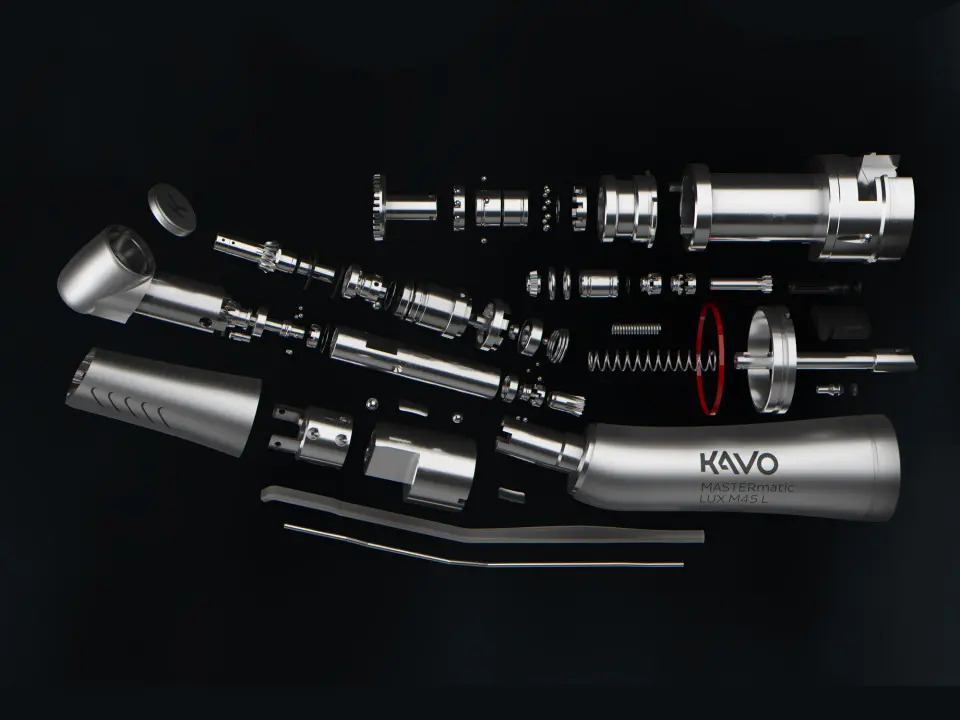
\includegraphics[width=\textwidth]{images/matermatic.jpg}
    \caption*{MASTERmatic LUX M45 L}
  \end{minipage}
  \hspace{0.05\textwidth}
  \begin{minipage}[b]{0.45\textwidth}
    \centering
    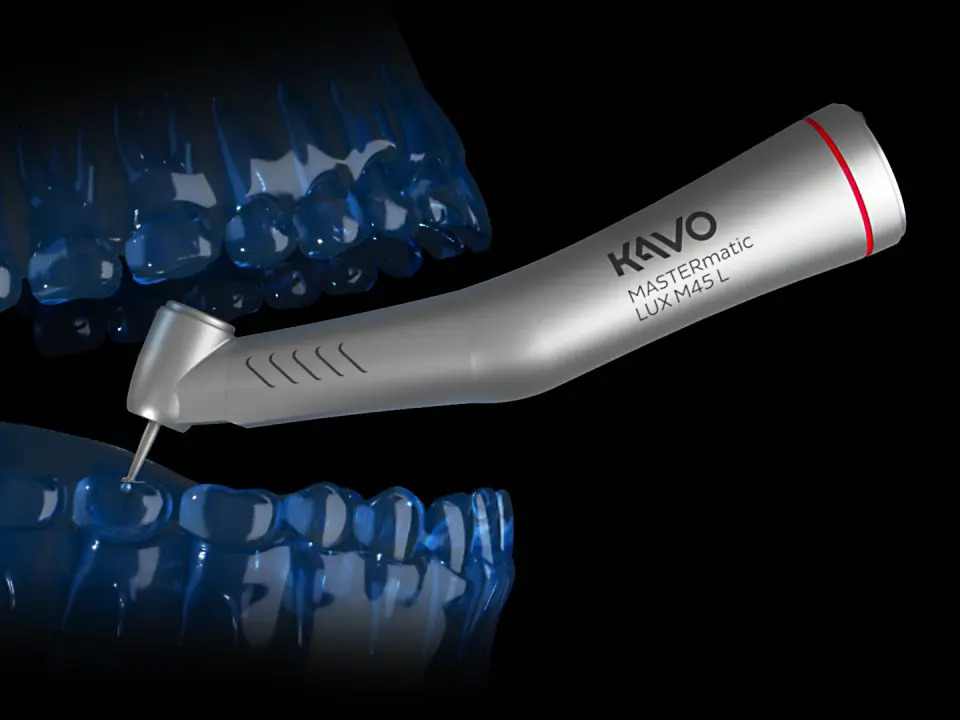
\includegraphics[width=\textwidth]{images/mastermatic2.jpg}
    \caption*{MASTERmatic LUX M45 L}
  \end{minipage}
  \caption{KaVo Handstücken und Winkelstücken}
  \label{fig:handstuecke}
\end{figure}
\vspace{1em}

\textbf{Turbinen (z.B. MASTERtorque M9000, EXPERTtorque E680):}

Turbinen bieten besonders hohe Drehzahlen und kommen vor allem bei der Kariesentfernung und Kronenpräparation zum Einsatz. Sie zeichnen sich durch geringe Geräuschentwicklung und hohe Effizienz aus.

\begin{figure}[H]
  \centering
  \begin{minipage}[b]{0.45\textwidth}
    \centering
    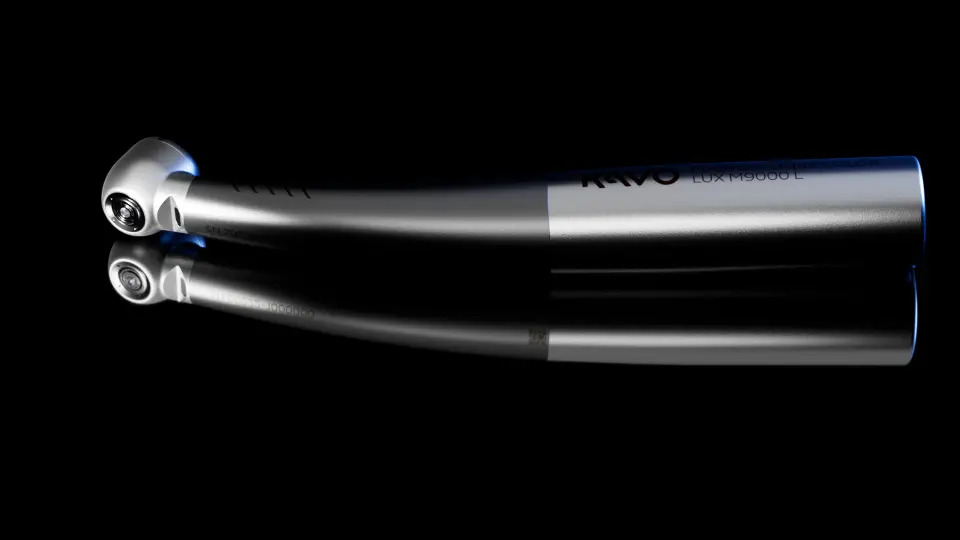
\includegraphics[width=\textwidth]{images/MASTERtorque-M9000-L_1-007-7100-black-cutout-3840px-2160px.jpg}
    \caption*{MASTERtorque M9000 L}
  \end{minipage}
  \hspace{0.05\textwidth}
  \begin{minipage}[b]{0.45\textwidth}
    \centering
    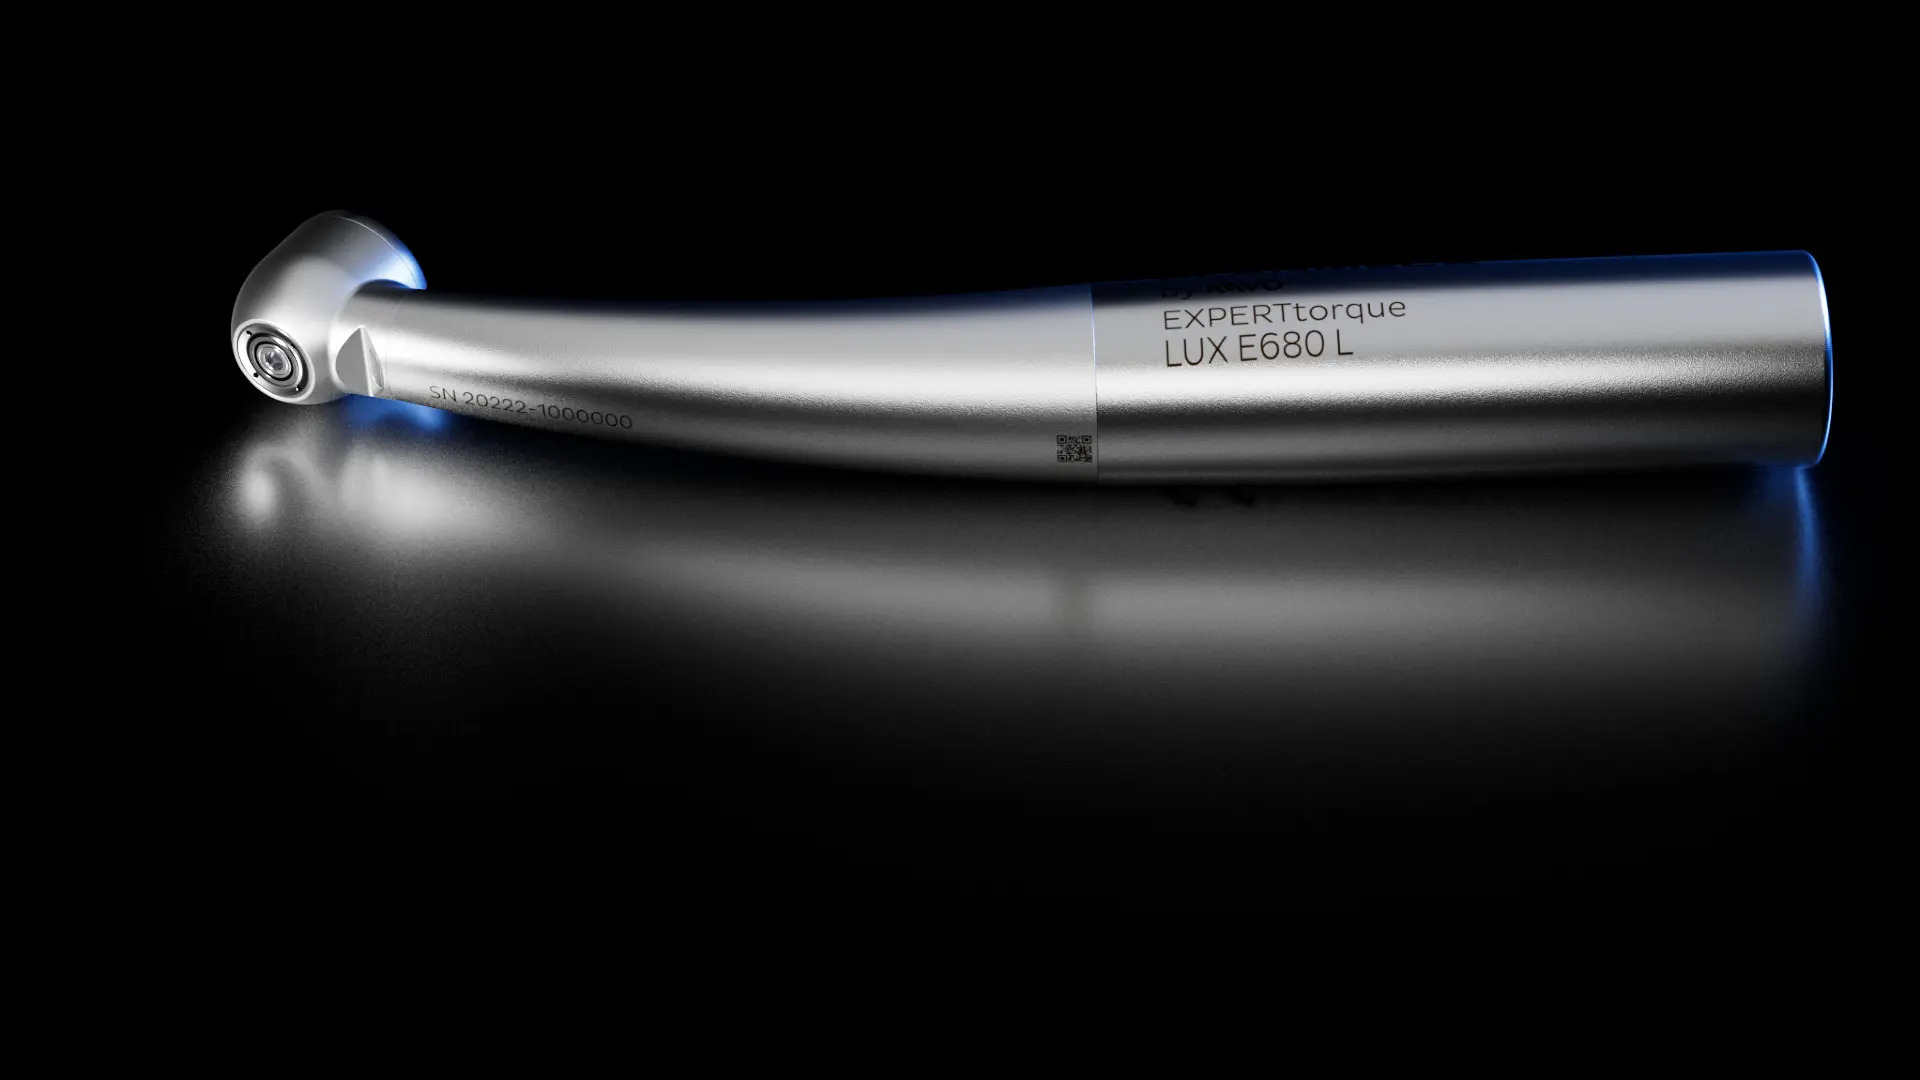
\includegraphics[width=\textwidth]{images/EXPERTtorque-LUX-Planmeca-E680L_1-015-0680-hb-v01-c-16-9-1920px-1080px.jpg}
    \caption*{EXPERTtorque™ E680}
  \end{minipage}
  \caption{KaVo Turbinen}
  \label{fig:Turbiene}
\end{figure}
\vspace{1em}

\textbf{Kupplungen, Motoren und LED-Systeme (z.B. MULTIflex™, INTRA LUX KL703 LED):}

Diese Komponenten verbinden Handstücke mit der Behandlungseinheit und versorgen sie mit Strom, Wasser, Luft und Licht. Die integrierten LEDs ermöglichen eine optimale Ausleuchtung des Arbeitsfeldes.

\begin{figure}[H]
  \centering
  \begin{minipage}[b]{0.45\textwidth}
    \centering
    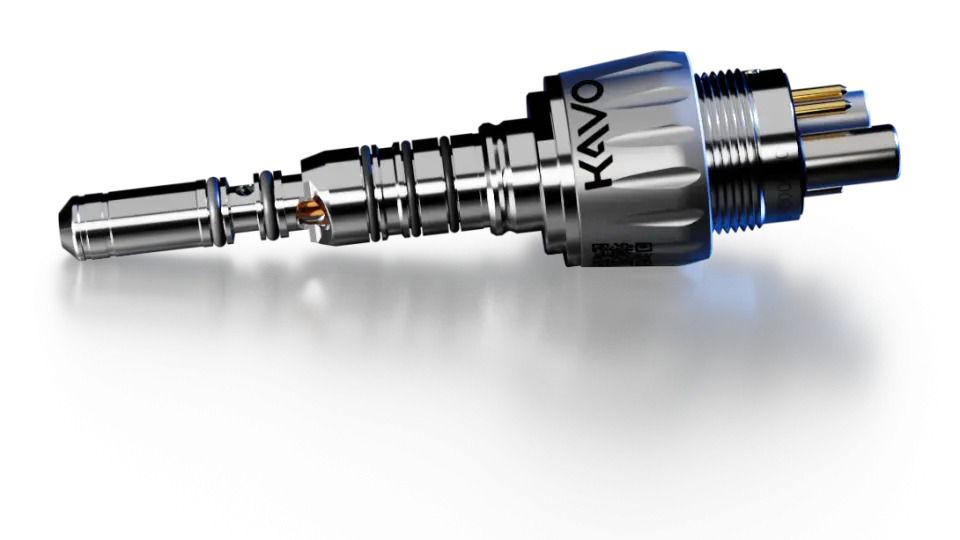
\includegraphics[width=\textwidth]{images/MULTIflex-465LED-transparent-1000px.jpg}
    \caption*{MULTIflex LED Kupplung 465 LED}
  \end{minipage}
  \hspace{0.05\textwidth}
  \begin{minipage}[b]{0.45\textwidth}
    \centering
    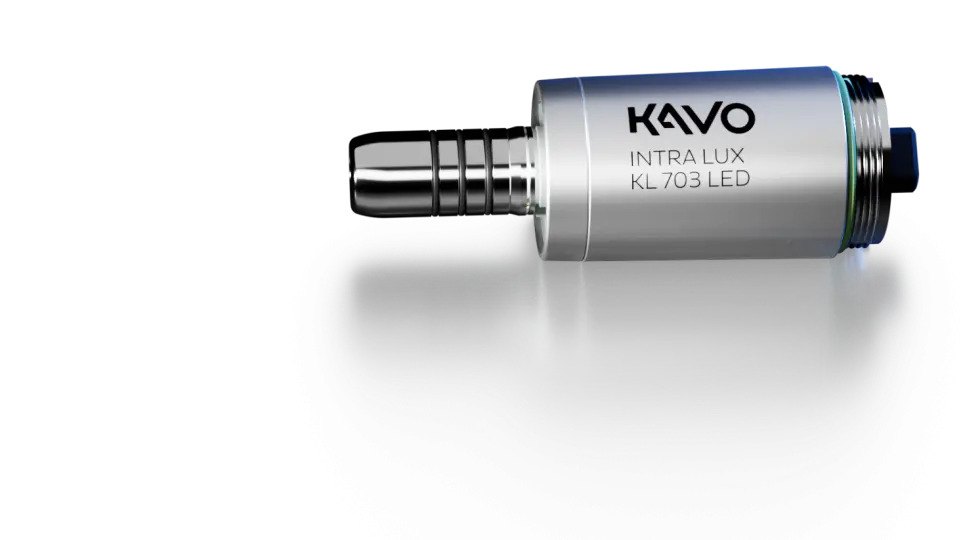
\includegraphics[width=\textwidth]{images/Motor-KL-703-LED_transparent-1000px.jpg}
    \caption*{INTRA LUX KL703 LED}
  \end{minipage}
  \caption{KaVo Kupplungen, Motoren und LED-Systeme}
  \label{fig:Kupplungen,Motoren und LED-Systeme}
\end{figure}
\vspace{1em}

\textbf{Scaler und Spitzen (z.B. SONICflex-Serie):}

Scaler werden zur Entfernung von Zahnstein und Belägen eingesetzt. Die SONICflex-Serie erlaubt eine sanfte und effektive Reinigung mit oszillierenden Bewegungen und verschiedenen Spitzenformen für unterschiedliche Indikationen.

\begin{figure}[H]
  \centering
  \begin{minipage}[b]{0.45\textwidth}
    \centering
    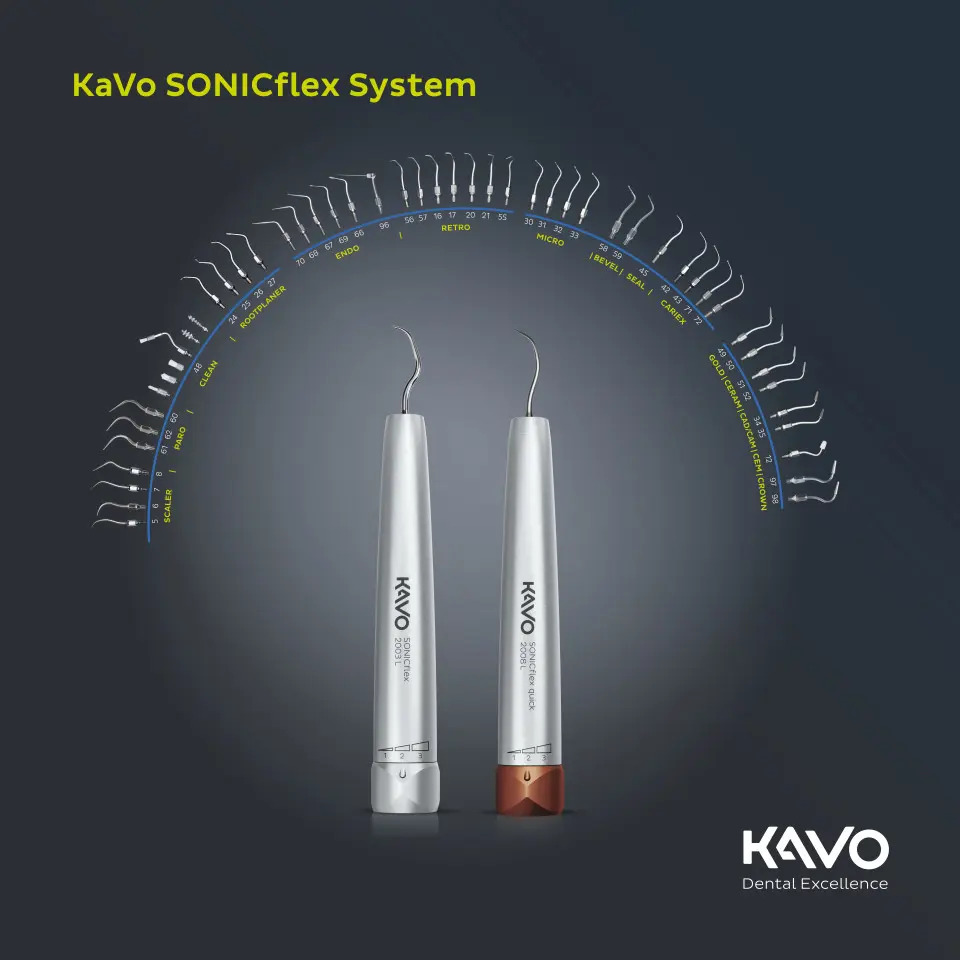
\includegraphics[width=\textwidth]{images/SONICflex_Spitzenkreis-dunkel_20210112_1000px.jpg}
    \caption*{SONICflex 2003 L / quick 2008 L}
  \end{minipage}
  \hspace{0.05\textwidth}
  \caption{KaVo Scaler und Spitzen}
  \label{fig:Scaler und Spitzen}
\end{figure}
\vspace{1em}

\textbf{Instrumente für Chirurgie und Endodontie:}

Diese Instrumente unterstützen chirurgische Eingriffe wie Extraktionen oder Knochenbearbeitungen sowie endodontische Behandlungen wie Wurzelkanalpräparation. Sie zeichnen sich durch hohe Präzision und spezielle Geometrien aus.

\begin{figure}[H]
  \centering
  \begin{minipage}[b]{0.45\textwidth}
    \centering
    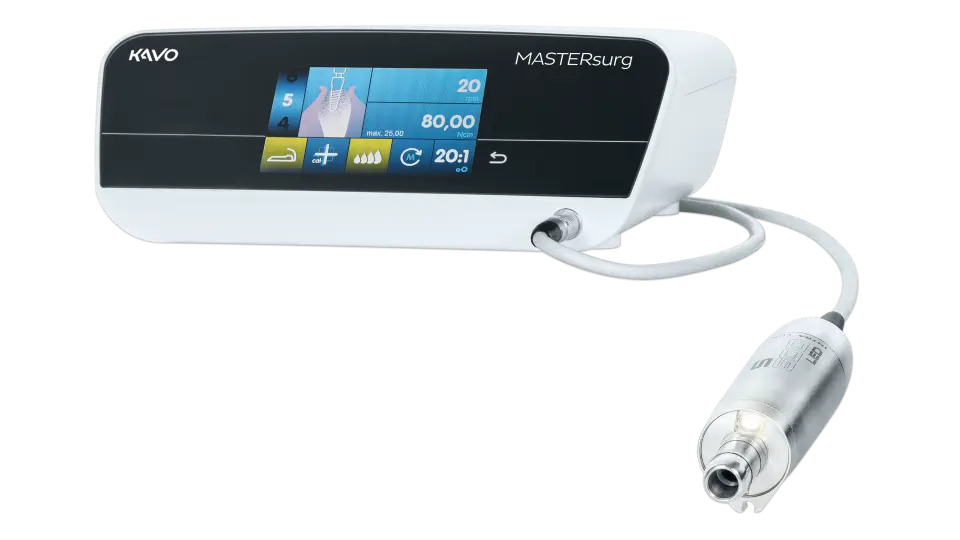
\includegraphics[width=\textwidth]{images/MASTERsurg_Motor_persp-transparent_3000px.jpg}
    \caption*{MASTERsurg LUX Wireless}
  \end{minipage}
  \hspace{0.05\textwidth}
  \begin{minipage}[b]{0.45\textwidth}
    \centering
    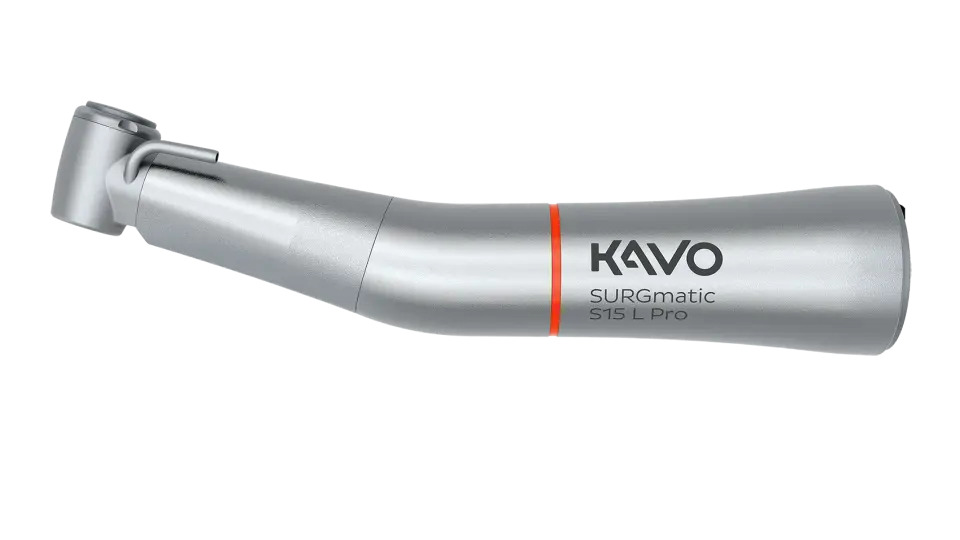
\includegraphics[width=\textwidth]{images/SURGmatic-S15L-Pro_transparent-1700px.jpg}
    \caption*{SURGmatic Winkelstück S15 L Pro}
  \end{minipage}
  \caption{KaVo Chirurgie und Endodontie Instrumente}
  \label{fig:Chirurgie und Endodontie Instrumente}
\end{figure}
\vspace{1em}

\textbf{Prophylaxe-Instrumente (z.B. PROPHYflex 4, perio tip, KaVo eSCALER):}

Mit dem PROPHYflex 4 und dem perio tip lassen sich Beläge und Verfärbungen gezielt entfernen – auch in schwer zugänglichen Bereichen. Der KaVo eSCALER arbeitet mit Ultraschalltechnologie zur schonenden Zahnsteinentfernung und unterstützt eine effiziente Prophylaxesitzung.

\begin{figure}[H]
  \centering
  \begin{minipage}[b]{0.45\textwidth}
    \centering
    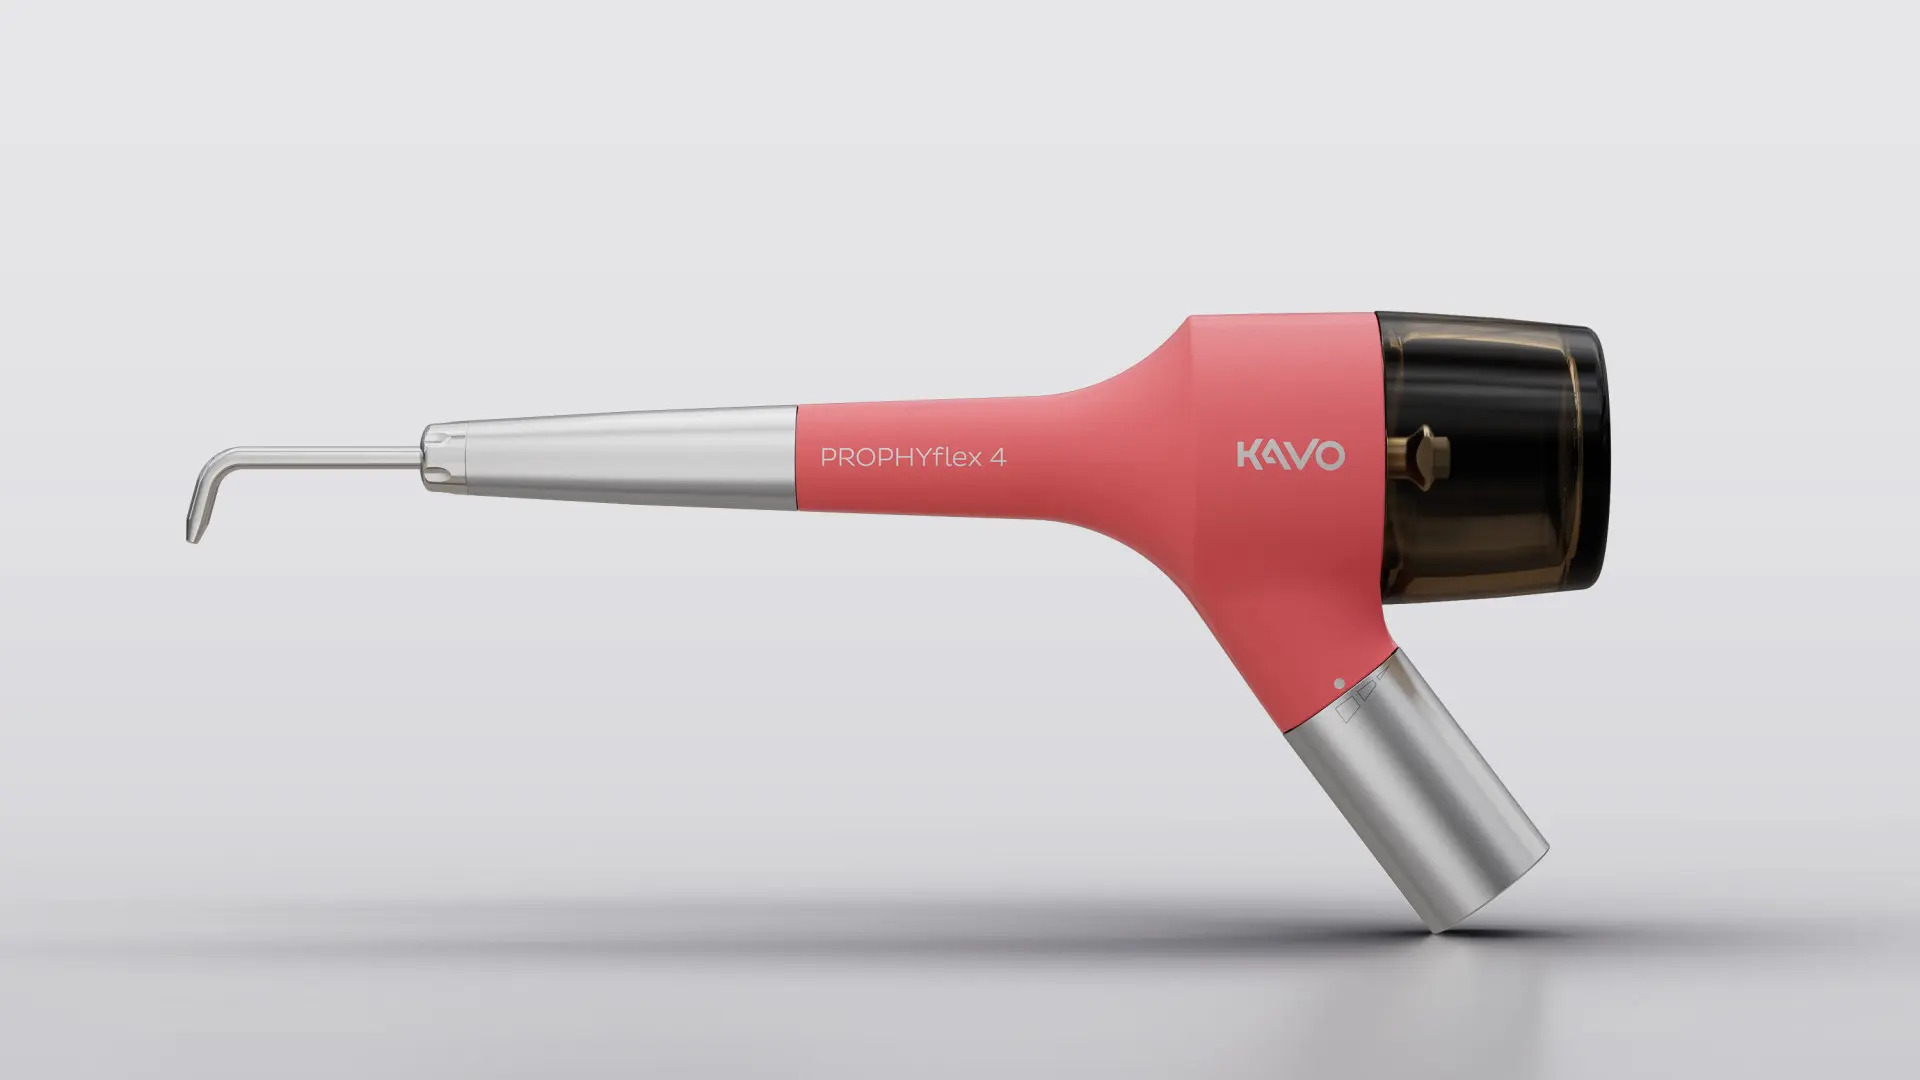
\includegraphics[width=\textwidth]{images/PROPHYflex-4-flaming_light_3000px.jpg}
    \caption*{PROPHYflex 4}
  \end{minipage}
  \hspace{0.05\textwidth}
  \begin{minipage}[b]{0.45\textwidth}
    \centering
    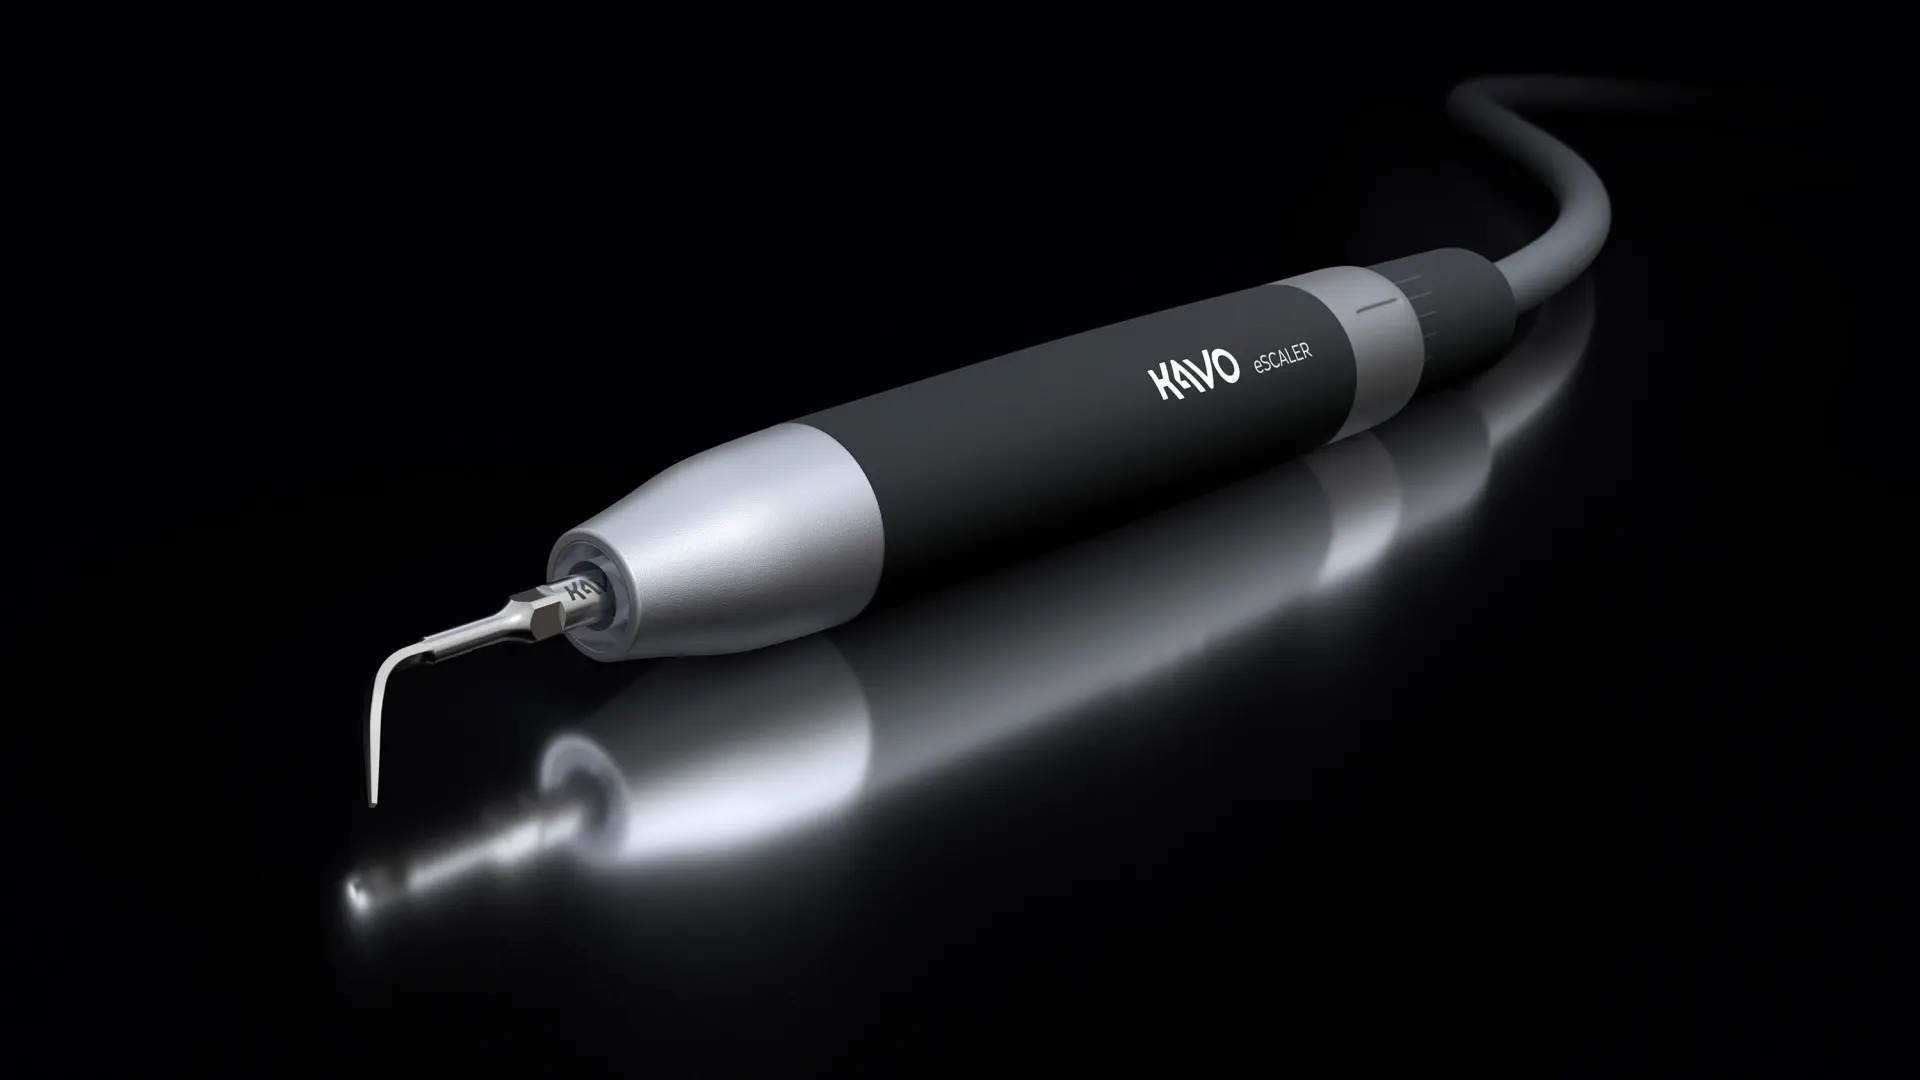
\includegraphics[width=\textwidth]{images/KaVo-eScaler-Ultrasonic-Scaler-Header_16-9.jpg}
    \caption*{KaVo eSCALER}
  \end{minipage}
  \caption{KaVo Prophylaxe-Instrumente}
  \label{fig:Prophylaxe-Instrumente}
\end{figure}
\vspace{1em}

\textbf{Restaurative Werkzeuge (z.B. RONDOflex, SONICflex retro/micro):}

Diese Instrumente ermöglichen minimalinvasive Präparationen, punktuelle Kariesbehandlung sowie die Reinigung von Fissuren. Die Pulverstrahl- und Ultraschalltechnik schont gesunde Zahnsubstanz.

\begin{figure}[H]
  \centering
  \begin{minipage}[b]{0.45\textwidth}
    \centering
    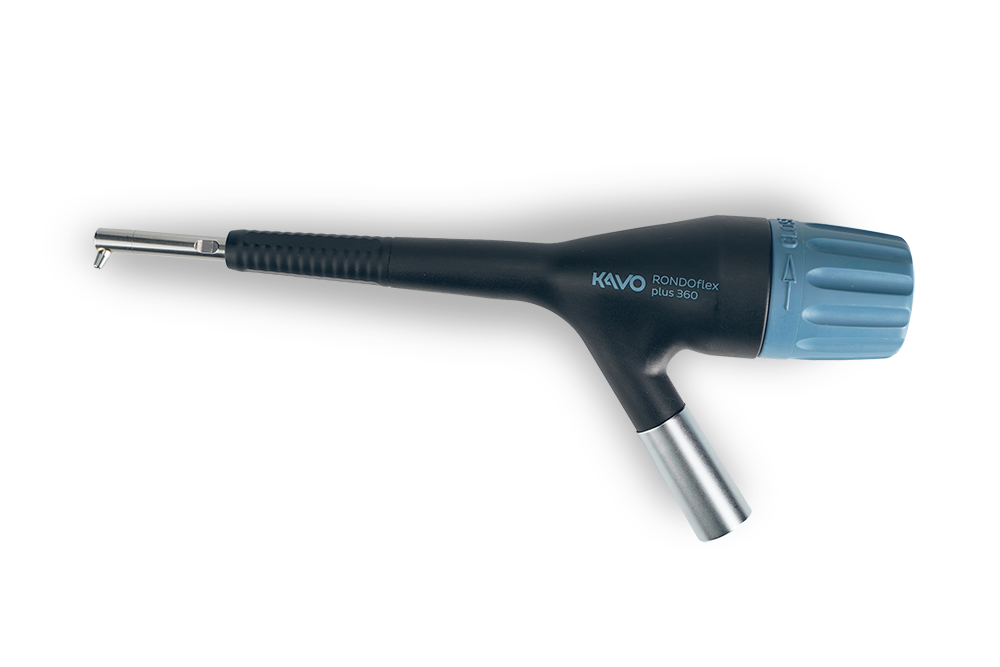
\includegraphics[width=\textwidth]{images/RONDOflex-plus-360.png}
    \caption*{RONDOflex plus 360}
  \end{minipage}
  \hspace{0.05\textwidth}
  \begin{minipage}[b]{0.45\textwidth}
    \centering
    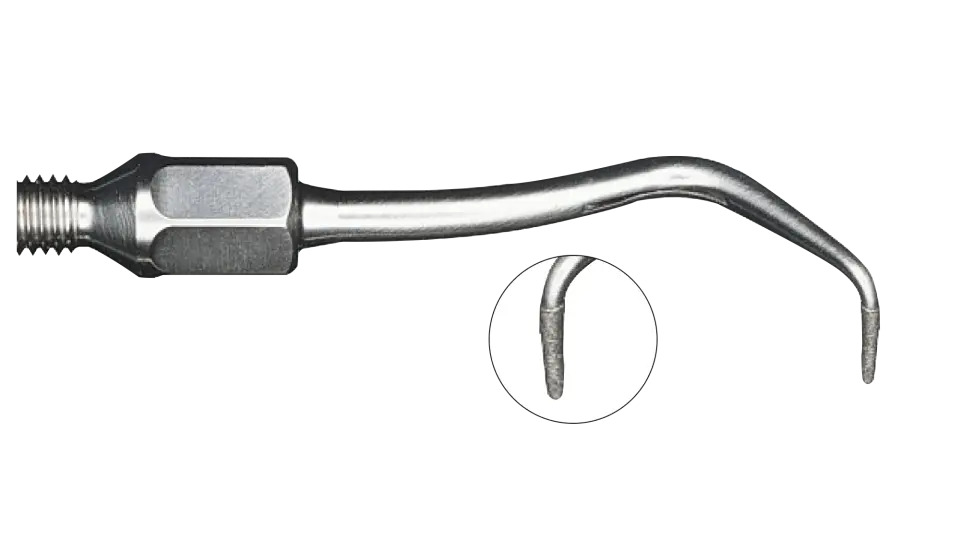
\includegraphics[width=\textwidth]{images/SONICflex-retro-Tip-Nr-56_transparent-16-9-2000px.jpg}
    \caption*{SONICflex retro Spitze Nr. 56}
  \end{minipage}
  \caption{KaVo Restaurative Werkzeuge}
  \label{fig:Restaurative Werkzeuge}
\end{figure}
\vspace{1em}

\subsubsection{KaVo Dentaleinheiten}

KaVo bietet Dentaleinheiten in verschiedenen Preiskategorien an – von wirtschaftlichen Einsteigermodellen bis hin zu hochwertigen Premiumlösungen. Dazu zählen unter anderem die \textit{ESTETICA E70/E80 Vision}, \textit{KaVo uniQa} und \textit{KaVo amiQa}, die sich durch ihre ergonomische Gestaltung, hochwertige Verarbeitung, umfangreiche Funktionalität und hohe Zuverlässigkeit auszeichnen. Sie bieten sowohl für Behandler als auch für Patienten höchsten Komfort und ermöglichen eine intuitive Steuerung aller Komponenten.

Moderne Features wie individuell programmierbare Behandlungspositionen, integrierte Hygienefunktionen, anpassbare Benutzeroberflächen sowie die nahtlose Einbindung von Diagnose- und Kommunikationssystemen unterstützen einen effizienten und digitalen Praxisablauf.
\vspace{1em}
\begin{figure}[H]
  \centering
  \begin{minipage}[b]{0.55\textwidth}
    \centering
    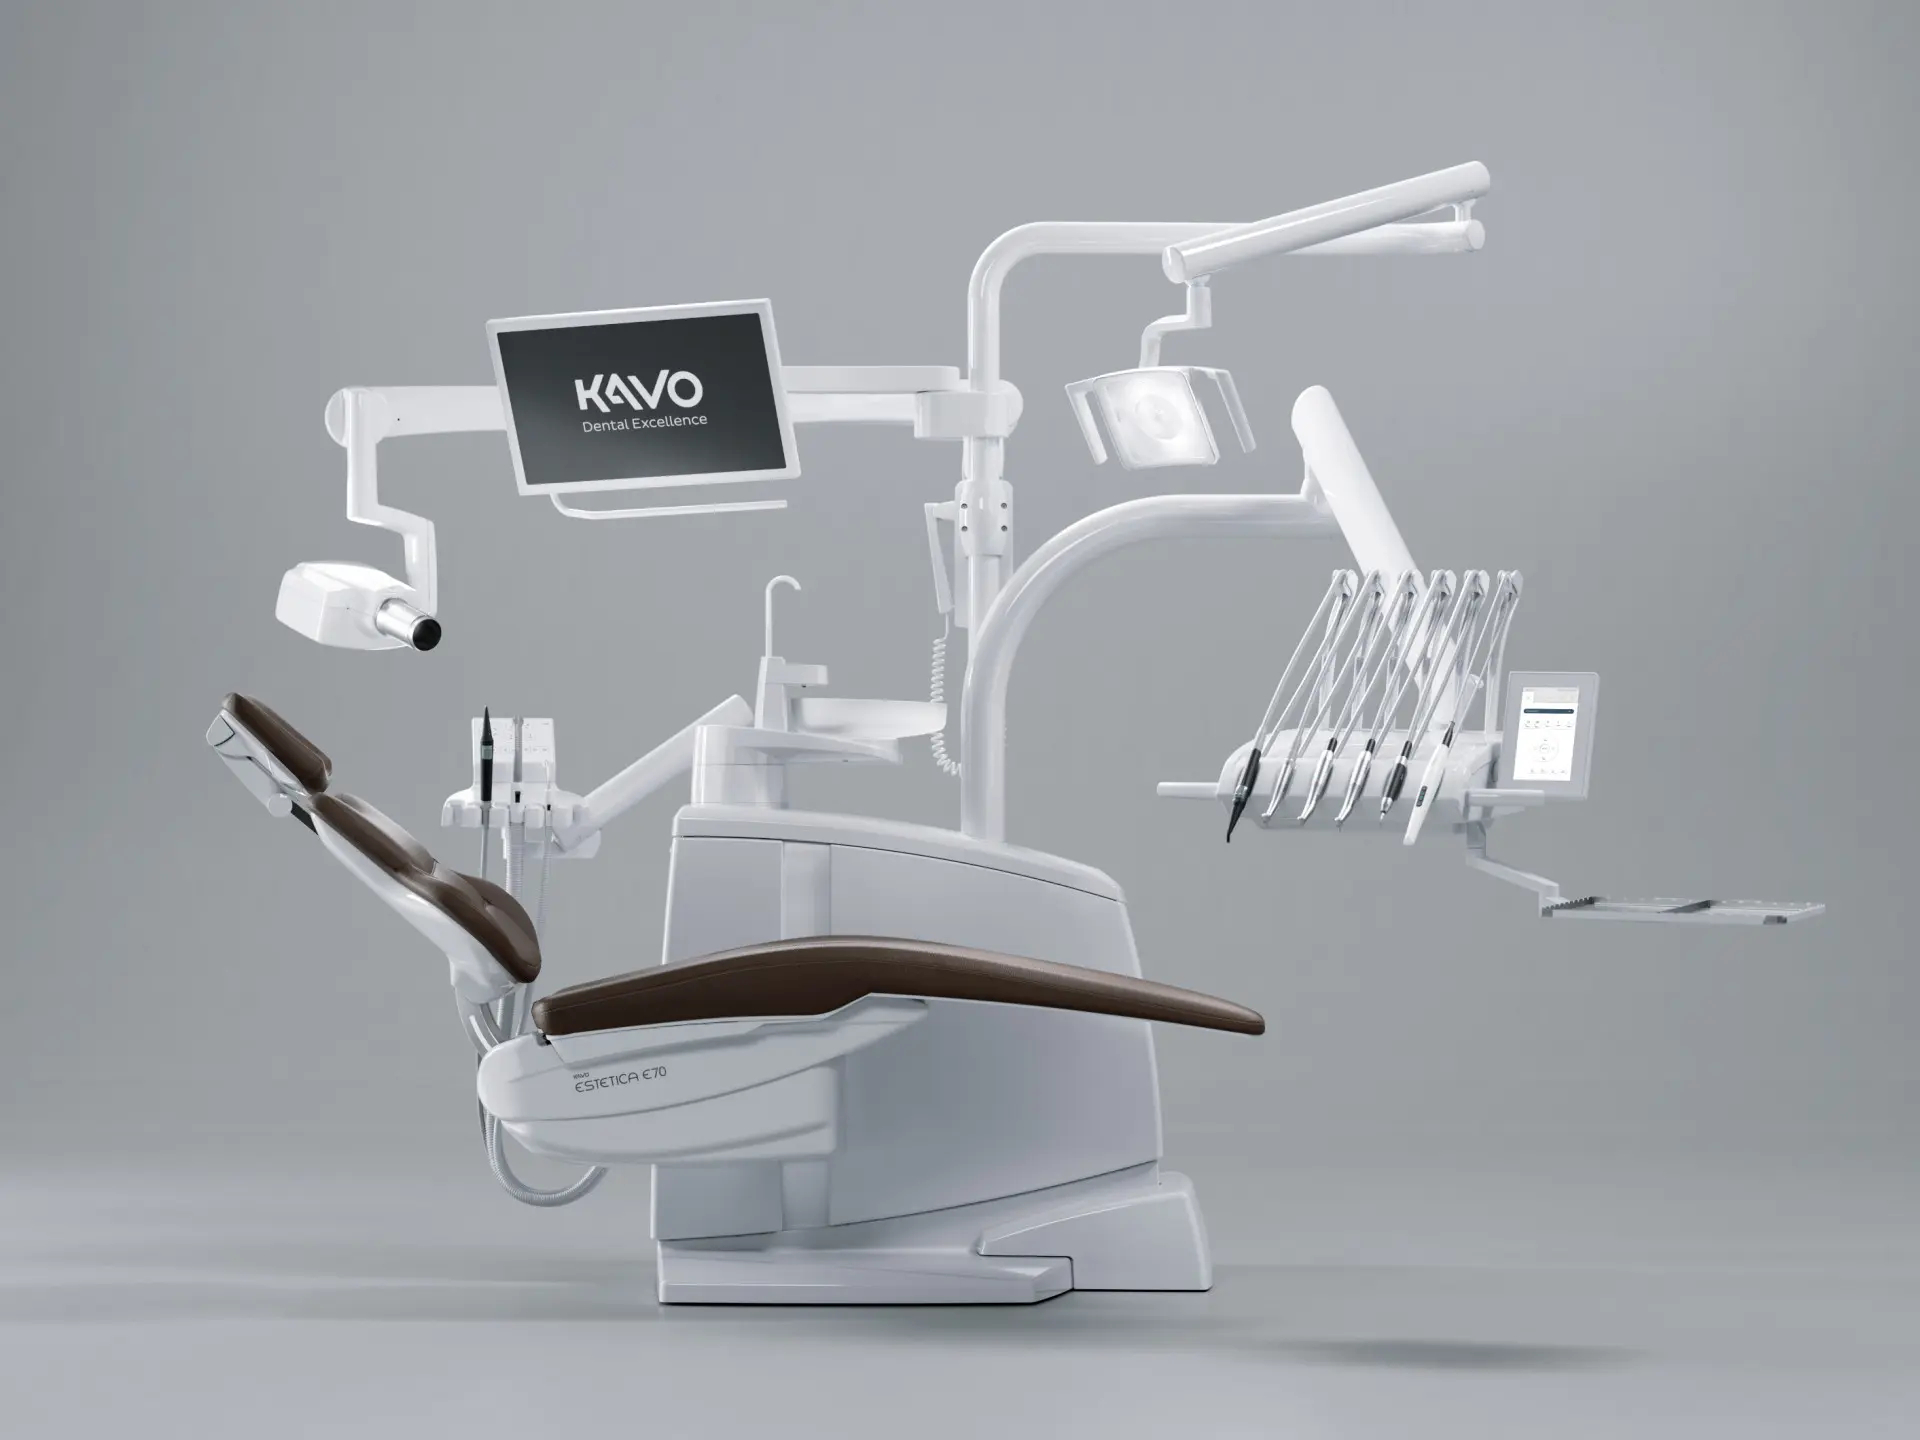
\includegraphics[width=\textwidth]{images/ESTETICA-E70-E80-S-coffeel-ProXam-front_3500px.jpg}
    
  \end{minipage}
  \hspace{0.05\textwidth}
  \caption{KaVo ESTETICA E70}
  \label{fig:Scaler und Spitzen}
\end{figure}
\vspace{1em}
\begin{figure}[H]
  \centering
  \begin{minipage}[b]{0.55\textwidth}
    \centering
    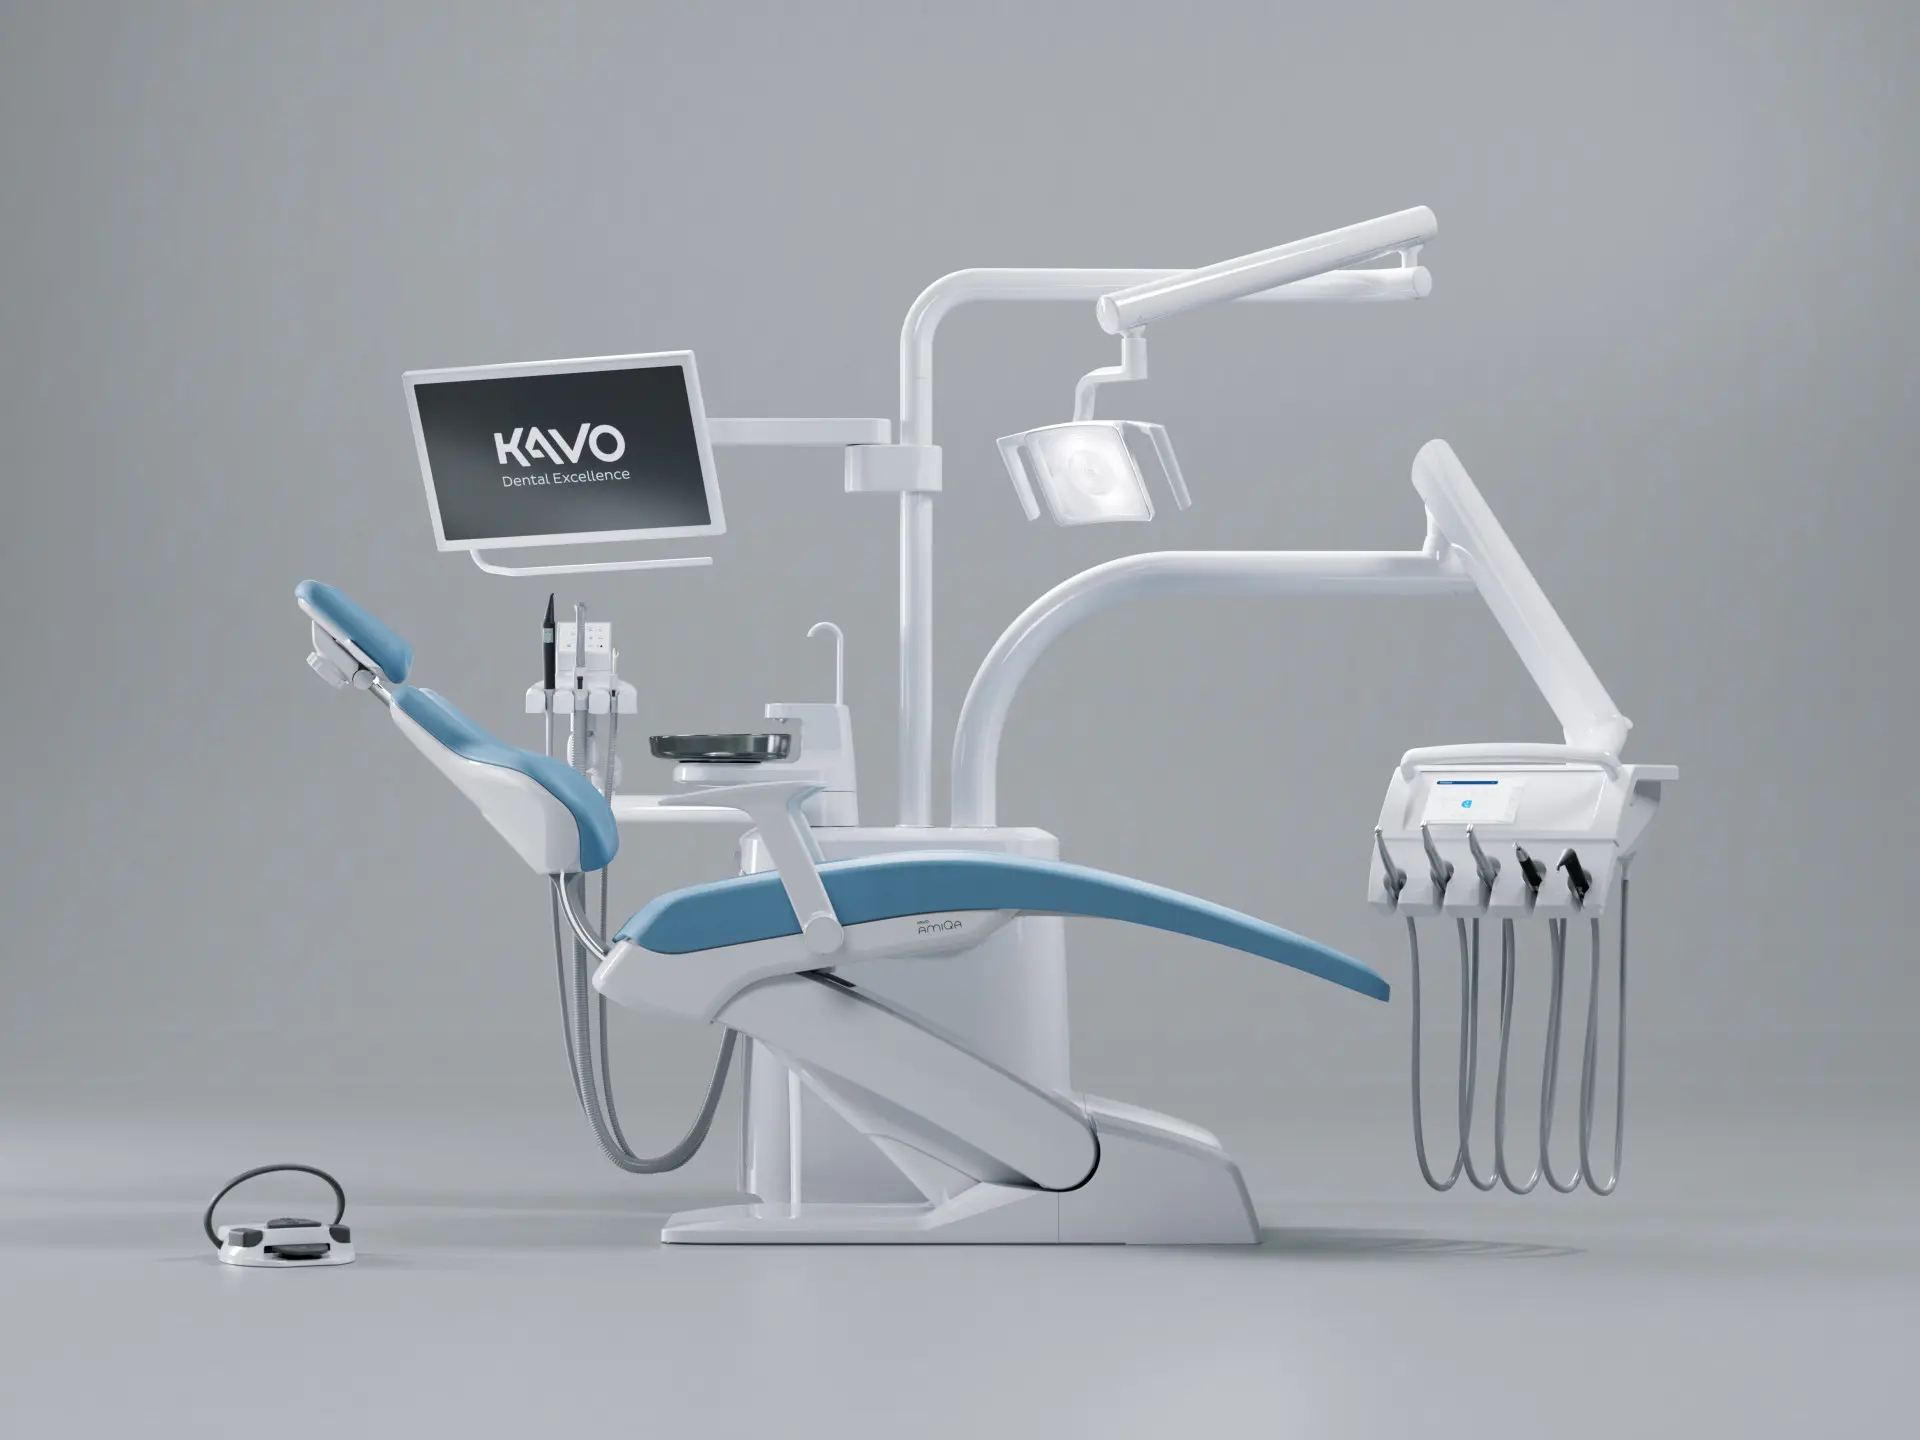
\includegraphics[width=\textwidth]{images/KaVo-amiQa-TM-frost_9clock-background.jpg}
    
  \end{minipage}
  \hspace{0.05\textwidth}
  \caption{KaVo amiQa}
  \label{fig:Scaler und Spitzen}
\end{figure}
\vspace{1em}
\subsubsection{Patientenkommunikation}

In modernen Zahnarztpraxen spielt die digitale Patientenkommunikation eine zentrale Rolle. Systeme wie \textit{CONNECTbase}, \textit{CONNECTLink} und \textit{CONEXIO} tragen dazu bei, intraorale Bild- und Videodaten effizient zu erfassen, lokal darzustellen und bei Bedarf in die zentrale Patientenakte zu integrieren.

\textit{CONNECTbase} ist eine Komplettlösung aus Hard- und Software, die auf einem eingebetteten Steuerrechner (z.\,B. Raspberry Pi Compute Module 4) basiert und unter Linux betrieben wird. Die Software besteht aus einer in C++ entwickelten Anwendung, die eine native Benutzeroberfläche bereitstellt. Über diese werden Livebilder der intraoralen Kamera (z.\,B. \textit{ProXam iCam} oder \textit{DIAGNOcam Vision Full HD}) auf dem Hauptbildschirm der Dentaleinheit angezeigt. Alle Inhalte, die auf dem Hauptbildschirm erscheinen, stammen direkt aus dieser nativen Schnittstelle.

Ergänzend zur nativen Anzeige bietet \textit{CONNECTbase} eine webbasierte Benutzeroberfläche, die über das separate Touchdisplay der Dentaleinheit aufgerufen werden kann. Diese Web-GUI ermöglicht es dem Benutzer, zwischen verschiedenen Anzeigemodi auf dem Hauptbildschirm zu wählen (z.\,B. Patientenbilder, Kamerastream) und darüber hinaus zentrale Einstellungen der Anwendung zu konfigurieren – etwa Hintergrundbild, Netzwerkeinstellungen oder Datenmanagement.


\textit{CONEXIO} und \textit{CONNECTLink} schließlich ist die zentrale Praxissoftware, die empfangene Bilddaten dauerhaft in der Patientenakte speichert, eine strukturierte Zuordnung zu Patienten ermöglicht und erweiterte Bildbearbeitungs-, Dokumentations- und Archivierungsfunktionen bietet. Somit stellen die sicher, dass alle relevanten visuellen Befunde aus der Behandlung — insbesondere Vorher-Nachher-Aufnahmen, Diagnosebilder und Fortschrittsdokumentationen — langfristig verfügbar sind.

\textit{ProXam iCam} ist eine intraorale Kamera zur Live-Darstellung von Zahnbefunden direkt am Behandlungsstuhl. Sie unterstützt eine transparente Kommunikation und erleichtert die visuelle Patientenaufklärung.

\textit{KaVo Screen} ist ein in die Einheit integrierter Bildschirm zur Darstellung von Bilddaten wie Röntgen- oder Kamerabildern. Er dient der effektiven Patientenberatung und fördert das Verständnis sowie die Akzeptanz von Behandlungsmaßnahmen.
\vspace{3em}
\begin{figure}[H]
  \centering
  \begin{minipage}[b]{0.45\textwidth}
    \centering
    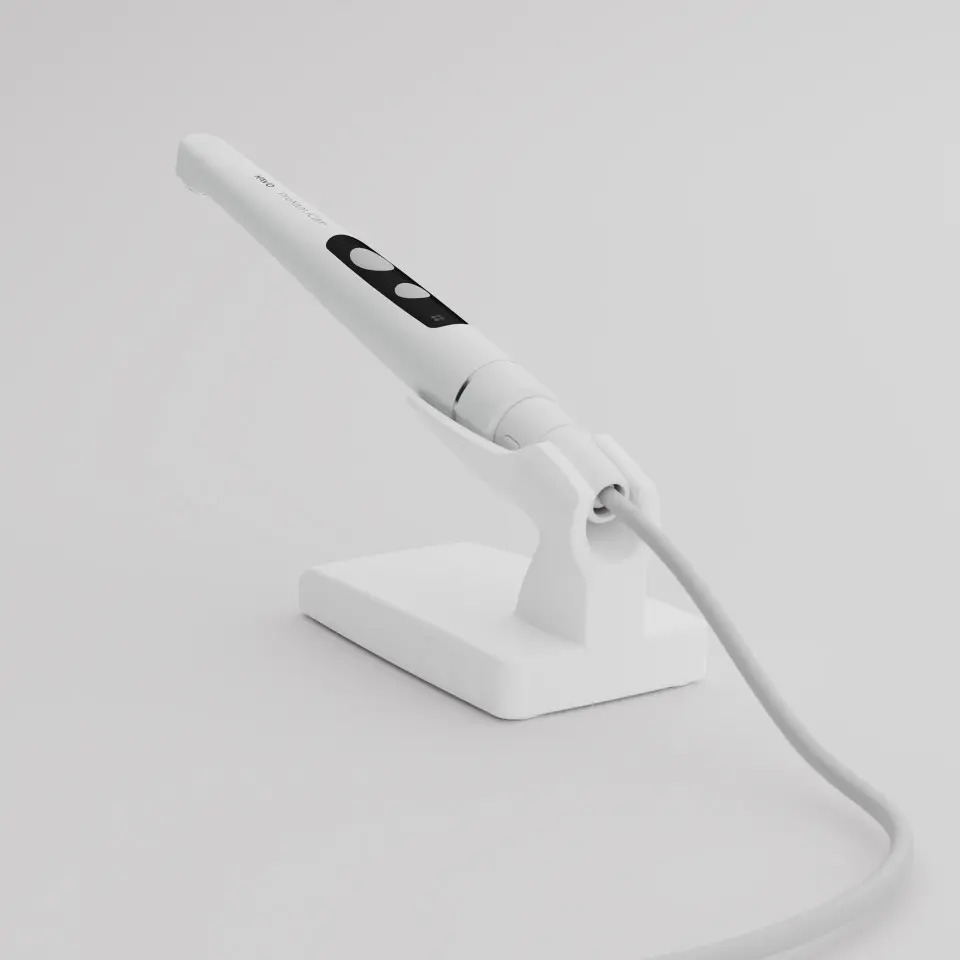
\includegraphics[width=\textwidth]{images/ProXam-iCam_table_background-1-1.jpg}
    \caption*{ProXam iCam}
  \end{minipage}
  \hspace{0.05\textwidth}
  \begin{minipage}[b]{0.45\textwidth}
    \centering
    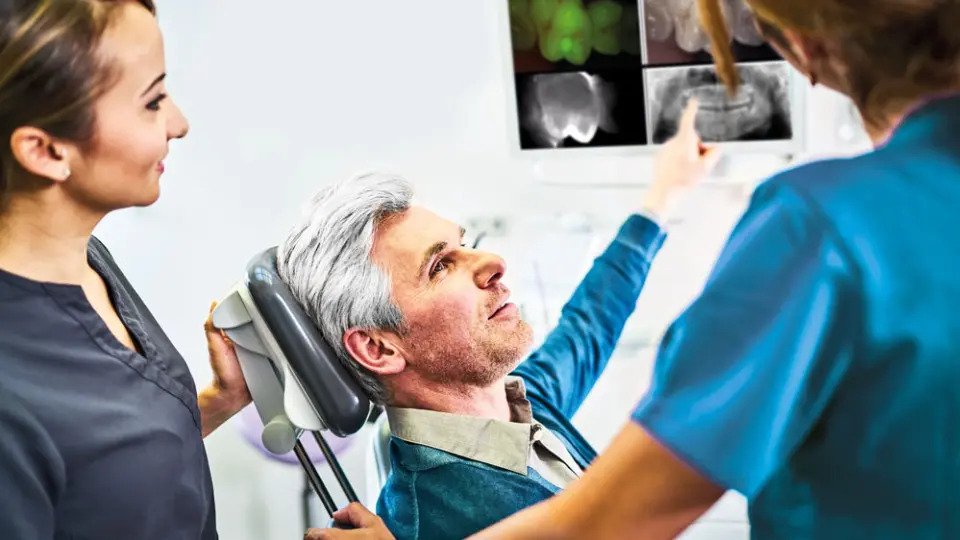
\includegraphics[width=\textwidth]{images/KaVo-uniQa_CONEXIO-Team_1000px.jpg}
    \caption*{KaVo Screen}
  \end{minipage}
  \caption{KaVo Patientenkommunikation}
  \label{fig:Patientenkommunikation und Vernetzung}
\end{figure}
\vspace{-1em}
\begin{figure}[H]
  \centering
  \begin{minipage}[b]{0.45\textwidth}
    \centering
    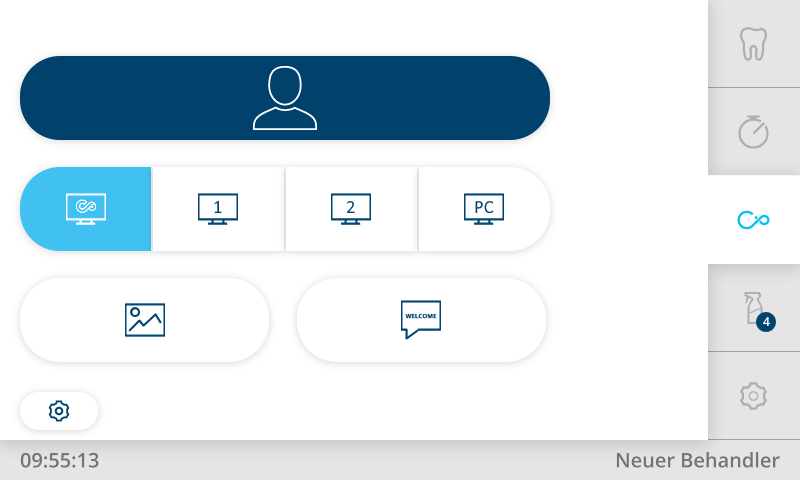
\includegraphics[width=\textwidth]{images/2025-07-23T09_55_13_796.png}
    \caption*{CONNECTbase auf touch display}
  \end{minipage}
  \hspace{0.05\textwidth}
  \begin{minipage}[b]{0.45\textwidth}
    \centering
    
\includegraphics[width=\textwidth]{images/Conexio-Logo_700px.jpg}
    \caption*{CONEXIO}
  \end{minipage}
  \caption{KaVo Vernetzungs Software}
  \label{fig:Vernetzung Software}
\end{figure}
\vspace{1em}

\subsubsection{Diagnostik und Bildgebung}

KaVo bietet fortschrittliche Technologien zur intra- und extraoralen Bildgebung, die eine präzise Diagnostik ermöglichen und somit eine fundierte Behandlungsplanung unterstützen.

\textbf{Intraorale Diagnosegeräte (z.B. DIAGNOcam Vision Full HD, DIAGNOdent pen):} \\
Diese Geräte ermöglichen eine strahlungsfreie, frühzeitige Karieserkennung direkt am Patienten. Die \textit{DIAGNOcam} nutzt das Prinzip der Transillumination mit sichtbarem Licht, während der \textit{DIAGNOdent pen} laserbasiert arbeitet und insbesondere versteckte Läsionen sichtbar macht.

\vspace{-1em}
\begin{figure}[H]
  \centering
  \begin{minipage}[b]{0.40\textwidth}
    \centering
    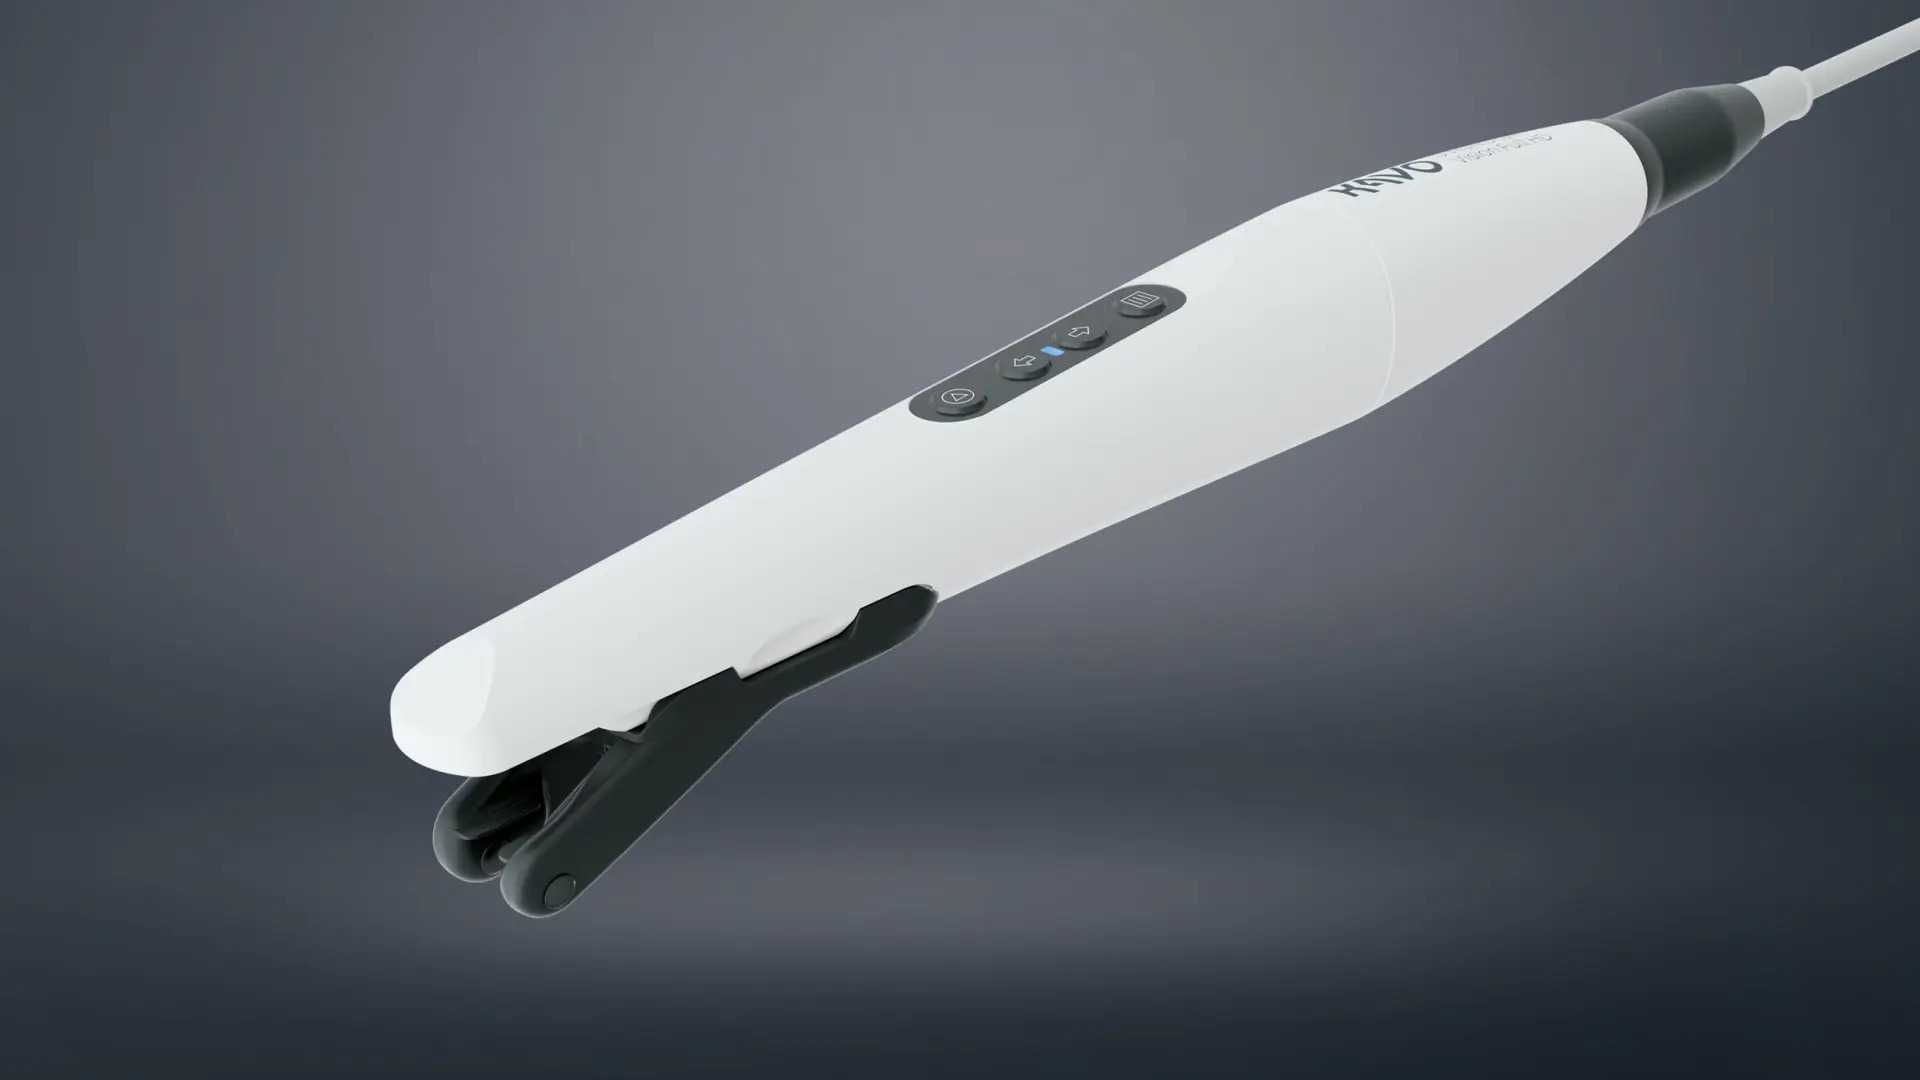
\includegraphics[width=\textwidth]{images/DIAGNOcam-Vision-Full-HD_Header-dark-V4_16-7-3840px.jpg}
    \caption*{DIAGNOcam Vision Full HD}
  \end{minipage}
  \hspace{0.05\textwidth}
  \begin{minipage}[b]{0.40\textwidth}
    \centering
    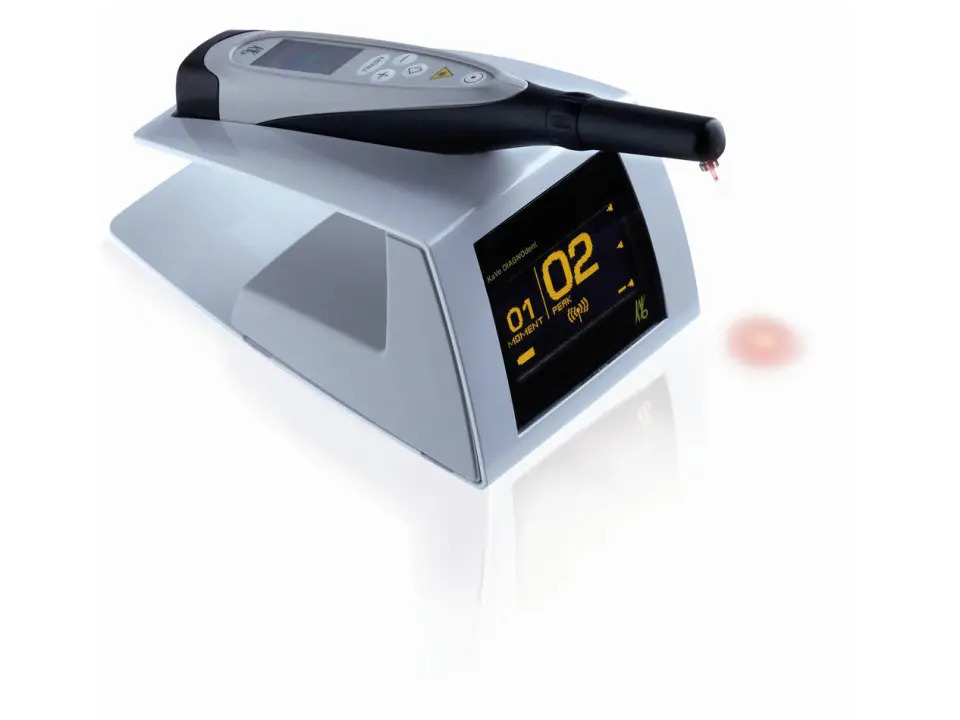
\includegraphics[width=\textwidth]{images/DIAGNOdent-pen_1809px.jpg}
    \caption*{DIAGNOdent pen}
  \end{minipage}
  \caption{KaVo Intraorale Diagnosegeräte}
  \label{fig:Intraorale Diagnosegeräte}
\end{figure}
\vspace{1em}

\textbf{Bildgebende Systeme (z.B. ProXam iX, 2D Pro):} \\
KaVo bietet sowohl intraorale als auch extraorale Bildgebungslösungen, die eine hohe Bildqualität und intuitive Bedienung vereinen. Diese Systeme unterstützen Diagnostik, Planung und Dokumentation.

\begin{figure}[H]
  \centering
  \begin{minipage}[b]{0.45\textwidth}
    \centering
    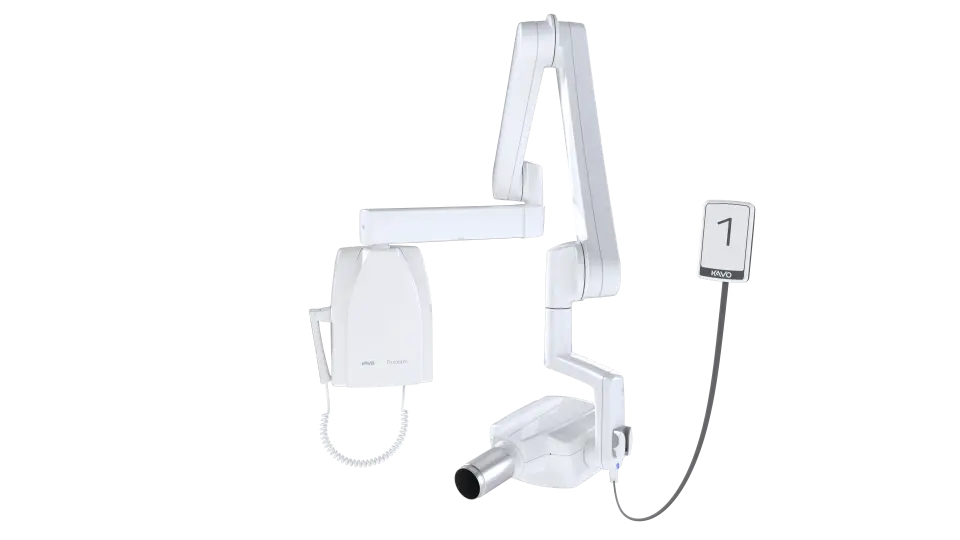
\includegraphics[width=\textwidth]{images/ProXam iX & iS.jpg}
    \caption*{ProXam iX}
  \end{minipage}
  \hspace{0.05\textwidth}
  \begin{minipage}[b]{0.45\textwidth}
    \centering
    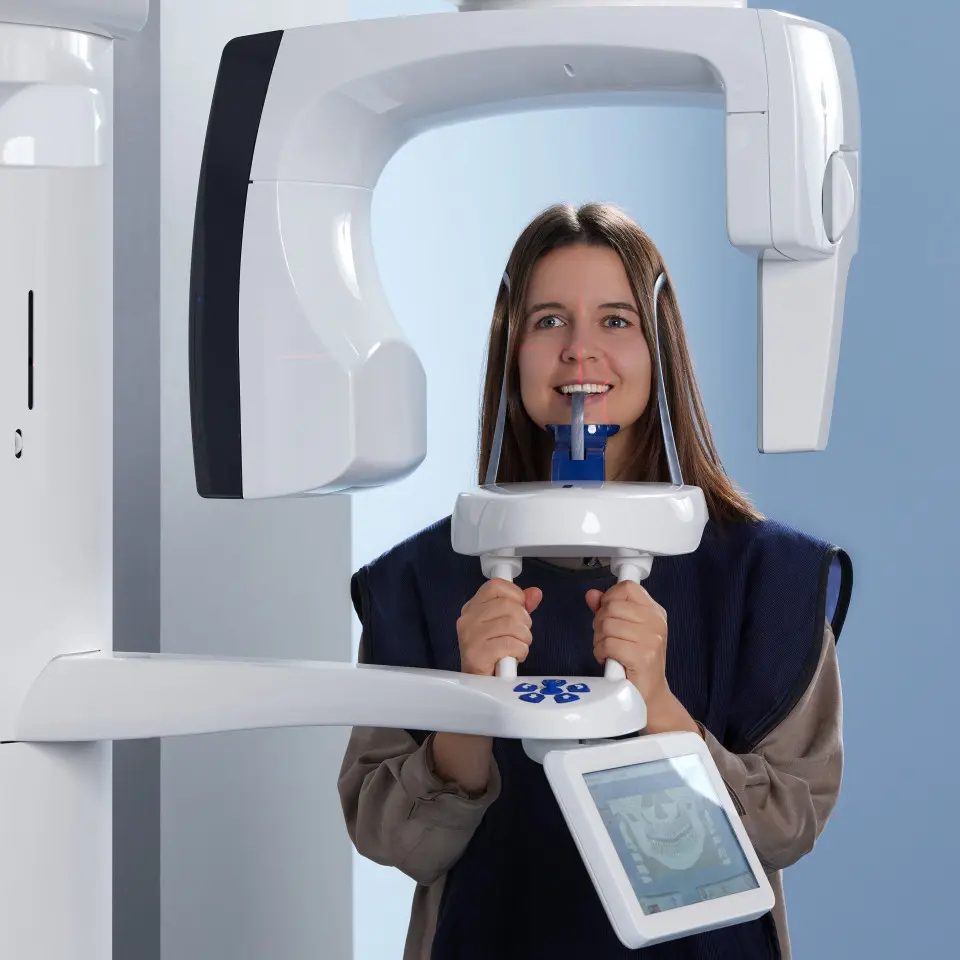
\includegraphics[width=\textwidth]{images/Extraoral-ProXam-2D_Patient-standing2_4000px.jpg}
    \caption*{ProXam 2D Pro}
  \end{minipage}
  \caption{KaVo Bildgebende Systeme}
  \label{fig:Bildgebende Systeme}
\end{figure}
\vspace{1em}

\textbf{Bildgebungssoftware (z.B. Romexis):} \\
Die Softwareplattform \textit{Romexis} integriert sich nahtlos in die Bildgebungshardware von KaVo und bietet umfassende Funktionen für Bildverarbeitung, Analyse und Datenverwaltung im digitalen Praxisworkflow.
\vspace{1em}
\begin{figure}[H]
  \centering
  \begin{minipage}[b]{0.35\textwidth}
    \centering
    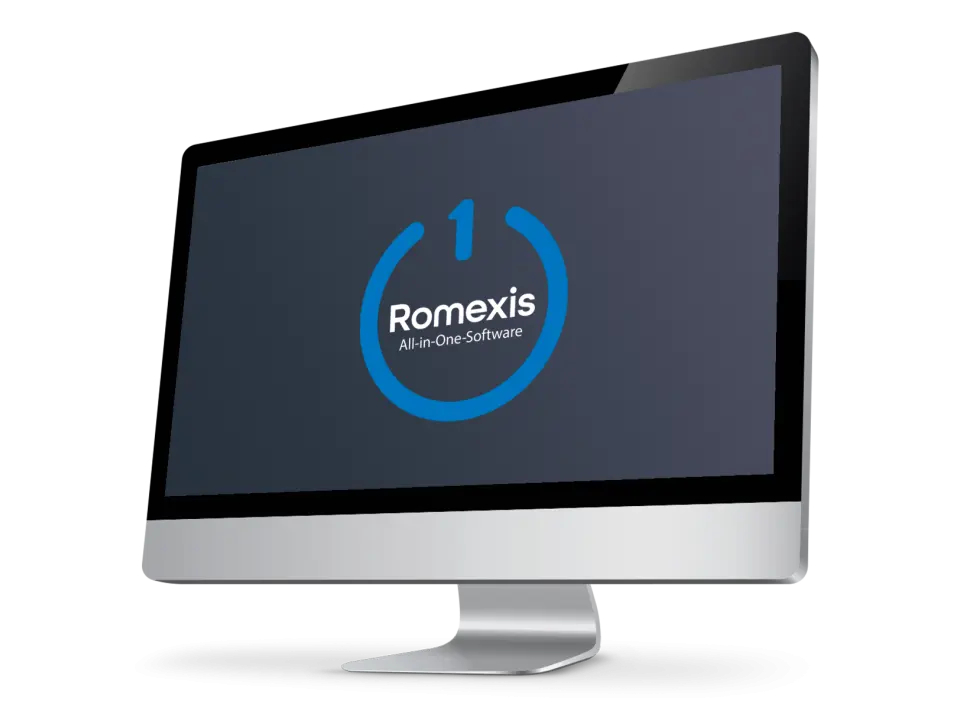
\includegraphics[width=\textwidth]{images/Romexis-Screen_2500px.jpg}
    \caption*{Romexis software}
  \end{minipage}
  \hspace{0.05\textwidth}
  \caption{KaVo Bildgebungssoftware}
  \label{fig:Bildgebungssoftware}
\end{figure}
\vspace{1em}

\subsubsection{Pflege, Reinigung und Hygiene}

Diese Kategorie umfasst Geräte und Produkte, die der Reinigung, Desinfektion und Pflege von Instrumenten und wasserführenden Systemen in Zahnarztpraxen dienen. Sie tragen entscheidend zur Einhaltung hoher Hygienestandards gemäß den Empfehlungen des Robert-Koch-Instituts (RKI) bei und unterstützen ein sicheres, zuverlässiges Praxisumfeld.
\newline
\newline
\newline
\textbf{Pflege- und Reinigungssysteme (z.\,B. QUATTROcare PLUS, CLEANspray, DRYspray):}

Zur effektiven Aufbereitung von Hand- und Winkelstücken sowie anderen Instrumenten bietet KaVo automatische und manuelle Lösungen. Das vollautomatische System \textit{QUATTROcare PLUS} übernimmt Reinigung, Schmierung und Trocknung in einem Zyklus. Ergänzend ermöglichen \textit{CLEANspray} und \textit{DRYspray} eine gezielte manuelle Nachbehandlung.

\begin{figure}[H]
  \centering
  \begin{minipage}[b]{0.45\textwidth}
    \centering
    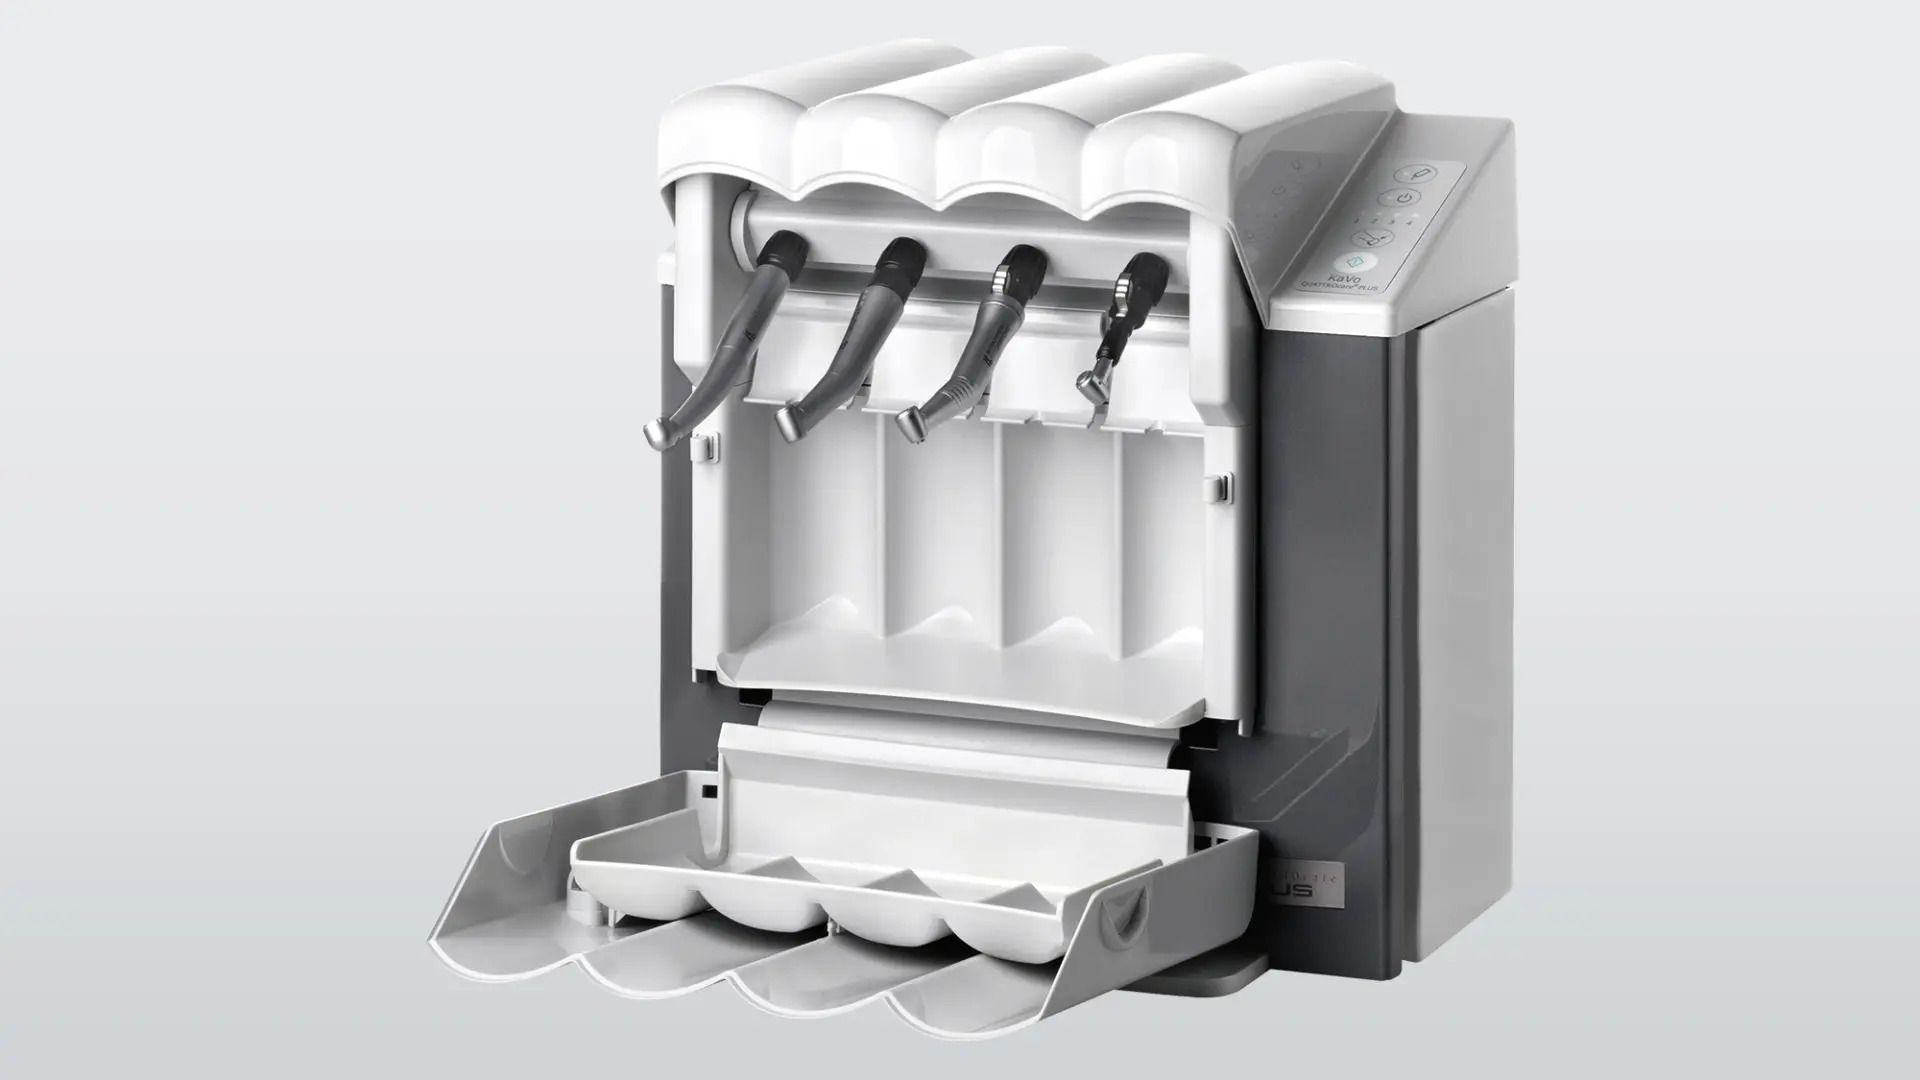
\includegraphics[width=\textwidth]{images/QUATTROcare-PLUS_open_16-9-2000px.jpg}
    \caption*{QUATTROcare PLUS}
  \end{minipage}
  \hspace{0.05\textwidth}
  \begin{minipage}[b]{0.45\textwidth}
    \centering
    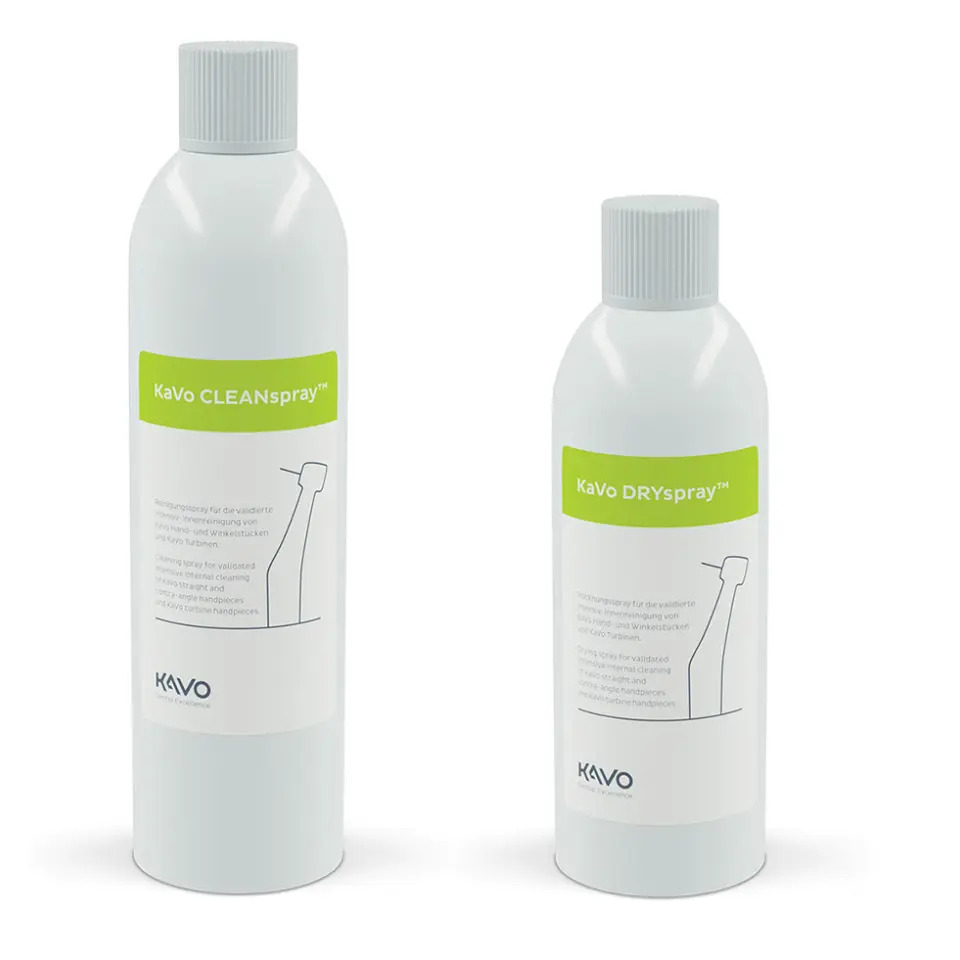
\includegraphics[width=\textwidth]{images/KaVo-CLEANspray-DRYspray.jpg}
    \caption*{CLEANspray \& DRYspray}
  \end{minipage}
  \caption{KaVo Pflege- und Reinigungssysteme für Dentalinstrumente}
  \label{fig:PflegeReinigung}
\end{figure}
\vspace{1em}




\textbf{Desinfektions- und Hygieneprodukte (z.\,B. DEKASEPTOL Gel, OXYGENAL 6):}

Für die regelmäßige Desinfektion von Absauganlagen und wasserführenden Leitungen kommen bewährte KaVo-Produkte zum Einsatz. \textit{DEKASEPTOL Gel} wird zur Reinigung von Absaugschläuchen verwendet, während \textit{OXYGENAL 6} speziell für die chemische Wasserhygiene entwickelt wurde.

\begin{figure}[H]
  \centering
  \begin{minipage}[b]{0.40\textwidth}
    \centering
    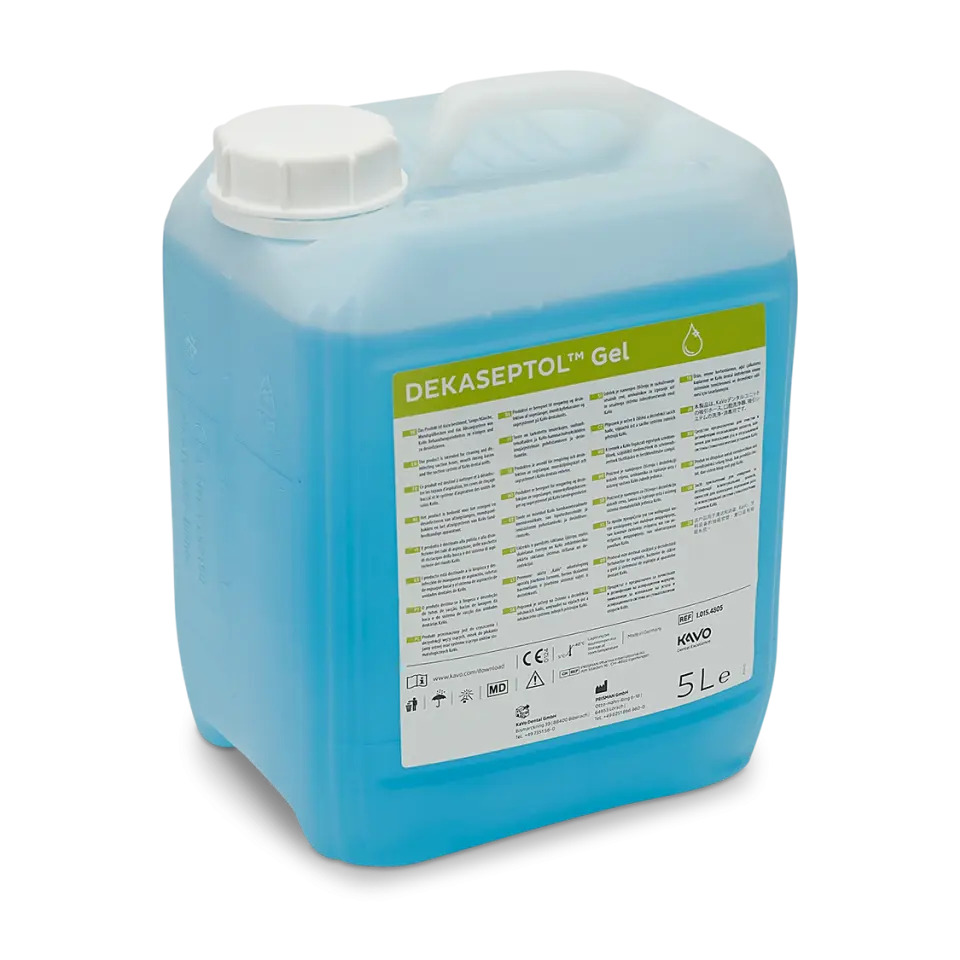
\includegraphics[width=\textwidth]{images/DEKASEPTOL-Gel_Nachfuellkanister_2000px.jpg}
    \caption*{DEKASEPTOL Gel}
  \end{minipage}
  \hspace{0.05\textwidth}
  \begin{minipage}[b]{0.40\textwidth}
    \centering
    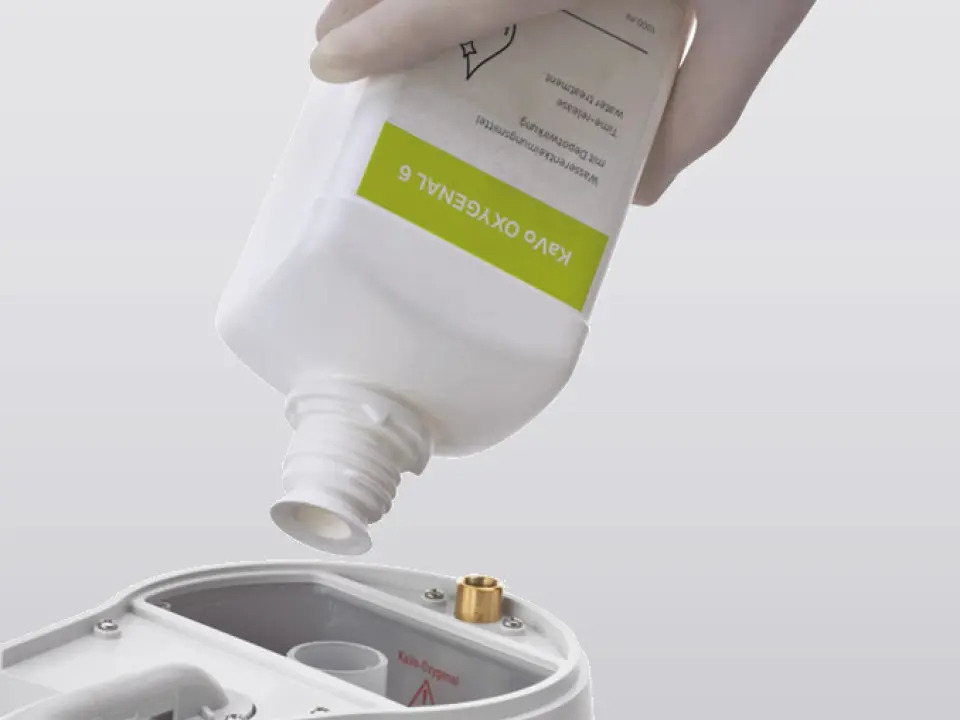
\includegraphics[width=\textwidth]{images/KaVo-Oxygenal_Handling_1000px.jpg}
    \caption*{OXYGENAL 6}
  \end{minipage}
  \caption{KaVo Desinfektions- und Hygieneprodukte}
  \label{fig:Hygieneprodukte}
\end{figure}
\vspace{1em}


\section{Projektauftrag und Kontext}

Im Rahmen meiner Bachelorarbeit bei KaVo Dental im Bereich \textit{Entwicklung Elektronik \& Medien} wurde untersucht, wie sich eine lokale, echtzeitfähige Kommunikationsschnittstelle zwischen KaVo-Dentaleinheiten und externen Systemen realisieren lässt. Ziel war es, auf dieser Basis wiederkehrende manuelle Abläufe – wie etwa Hygieneprozesse – durch externe Automatisierung zu unterstützen und so die Effizienz und Bedienfreundlichkeit in der zahnärztlichen Praxis und Kliniken zu verbessern.

Ein zentrales Anliegen bestand darin, eine Lösung zu entwickeln, die \textbf{ausschließlich lokal betrieben wird – ohne Cloud oder externe Serverinfrastruktur}. Die prototypische Umsetzung erfolgte durch die Integration der bestehenden Benutzeroberfläche \textit{CONNECTbase} mit der Open-Source-Plattform \textit{Home Assistant}, wodurch eine flexible und praxisnahe Automatisierung ermöglicht werden konnte.

Diese Arbeit dokumentiert den gesamten Entwicklungsprozess – von der Systemanalyse über die Auswahl geeigneter Technologien bis hin zur technischen Umsetzung und Bewertung des entwickelten Prototyps.

\textbf{Die zugrunde liegende Motivation für eine solche Lösung sowie die konkrete Herleitung der Anforderungen und Architekturentscheidungen werden in Kapitel~\ref{chap:projektkontext} ausführlich behandelt.}

